\documentclass[11pt]{article}

\usepackage[final]{acl}
\usepackage{times}
\usepackage{latexsym}
\usepackage[T1]{fontenc}
\usepackage[utf8]{inputenc}
\usepackage{microtype}
\usepackage{inconsolata}
\usepackage{graphicx}
\usepackage{booktabs}
\usepackage{multirow}
\usepackage{amsmath}
\usepackage{amssymb}
\usepackage{xcolor}
\usepackage{enumitem}

\newcommand{\PAhalf}{PA$_{1/2}$}

\title{AmanaMT: Translation Direction, Label Quality, and Automatic Metric Reliability}

\author{Isaac Thompson \\
  Brigham Young University \\
  \texttt{it238@byu.edu} \And
  Eric Ringger \\
  Brigham Young University}

\begin{document}
\maketitle
% AUTO-GENERATED by scripts/render_macros.py — DO NOT EDIT BY HAND
% Single source of truth: results/paper_stats.json
% To change a value: fix the analysis script that produced it, rerun the
% full pipeline (see this script's docstring), then rerun render_macros.py.
%
\newcommand{\BaselineValCoreMinPearson}{0.932}  % wmt_baseline_validation_segment_level.csv
\newcommand{\BaselineValCoreMinSpearman}{0.943}  % wmt_baseline_validation_segment_level.csv
\newcommand{\BaselineValMinPearson}{0.621}  % wmt_baseline_validation_segment_level.csv
\newcommand{\BaselineValMinSpearman}{0.650}  % wmt_baseline_validation_segment_level.csv
\newcommand{\BaselineValNChecks}{8}  % wmt_baseline_validation_segment_level.csv
\newcommand{\BeatsCometEntoXAgglutin}{6}  % recompute:table4_wins
\newcommand{\BeatsCometEntoXFusional}{7}  % recompute:table4_wins
\newcommand{\BeatsCometEntoXTotal}{13}  % recompute:table4
\newcommand{\BeatsCometXtoEnAgglutin}{6}  % recompute:table4_wins
\newcommand{\BeatsCometXtoEnFusional}{6}  % recompute:table4_wins
\newcommand{\BeatsCometXtoEnIsolating}{1}  % recompute:table4_wins
\newcommand{\CellCIEntoXAgglutinHi}{1.00}  % direction_separated_cell_cis.csv
\newcommand{\CellCIEntoXAgglutinLo}{0.54}  % direction_separated_cell_cis.csv
\newcommand{\CellCIEntoXFusionalHi}{1.00}  % direction_separated_cell_cis.csv
\newcommand{\CellCIEntoXFusionalLo}{0.59}  % direction_separated_cell_cis.csv
\newcommand{\CellCIXtoEnAgglutinHi}{1.00}  % direction_separated_cell_cis.csv
\newcommand{\CellCIXtoEnAgglutinLo}{0.54}  % direction_separated_cell_cis.csv
\newcommand{\CellCIXtoEnFusionalHi}{0.96}  % direction_separated_cell_cis.csv
\newcommand{\CellCIXtoEnFusionalLo}{0.29}  % direction_separated_cell_cis.csv
\newcommand{\ChrFErrorFreeDE}{0.74}  % surface_similarity.csv
\newcommand{\ChrFErrorFreeHE}{0.76}  % surface_similarity.csv
\newcommand{\CometXcometHeEsMinRho}{0.77}  % recompute:gemba_remap_check
\newcommand{\CsEnDelta}{+0.012}  % simpsons_cs_da.csv
\newcommand{\CsEnPooled}{.288}  % simpsons_cs_da.csv
\newcommand{\CsEnRangeHi}{0.69}  % simpsons_cs_da.csv
\newcommand{\CsEnRangeLo}{-0.01}  % simpsons_cs_da.csv
\newcommand{\DeDelta}{-0.001}  % tier_anomaly.csv
\newcommand{\DeEnCOMETRho}{.383}  % scores_de_en.csv
\newcommand{\DeEnCOMETRhoTbl}{0.383}  % scores_de_en.csv
\newcommand{\DeEnKiwiRho}{.414}  % scores_de_en.csv
\newcommand{\DeEnKiwiRhoTbl}{0.414}  % scores_de_en.csv
\newcommand{\DeEnMetricXRho}{.401}  % scores_de_en.csv
\newcommand{\DeEnN}{134{,}792}  % scores_de_en.csv
\newcommand{\DeRangeHi}{0.50}  % tier_anomaly.csv
\newcommand{\DeRangeLo}{0.32}  % tier_anomaly.csv
\newcommand{\DeWmtTwoOneRho}{.323}  % tier_anomaly.csv
\newcommand{\DeWmtTwoTwoRho}{.456}  % tier_anomaly.csv
\newcommand{\DeWmtTwoZeroRho}{.497}  % tier_anomaly.csv
\newcommand{\DiDValue}{0.065}  % recompute:gaps
\newcommand{\DirMetricBLEUEntoX}{0.319}  % recompute:direction_metric
\newcommand{\DirMetricBLEUPivot}{0.202}  % recompute:direction_metric
\newcommand{\DirMetricBLEUXtoEn}{0.223}  % recompute:direction_metric
\newcommand{\DirMetricCKXXIIIEntoX}{0.657}  % recompute:direction_metric
\newcommand{\DirMetricCKXXIIIPivot}{0.332}  % recompute:direction_metric
\newcommand{\DirMetricCKXXIIIXtoEn}{0.384}  % recompute:direction_metric
\newcommand{\DirMetricCOMETEntoX}{0.608}  % recompute:direction_metric
\newcommand{\DirMetricCOMETPivot}{0.354}  % recompute:direction_metric
\newcommand{\DirMetricCOMETXtoEn}{0.353}  % recompute:direction_metric
\newcommand{\DirMetricChrFEntoX}{0.383}  % recompute:direction_metric
\newcommand{\DirMetricChrFPivot}{0.247}  % recompute:direction_metric
\newcommand{\DirMetricChrFXtoEn}{0.252}  % recompute:direction_metric
\newcommand{\DirMetricMetricXEntoX}{0.698}  % recompute:direction_metric
\newcommand{\DirMetricMetricXPivot}{0.548}  % recompute:direction_metric
\newcommand{\DirMetricMetricXXtoEn}{0.391}  % recompute:direction_metric
\newcommand{\DirMetricxCOMETEntoX}{0.609}  % recompute:direction_metric
\newcommand{\DirMetricxCOMETPivot}{0.340}  % recompute:direction_metric
\newcommand{\DirMetricxCOMETXtoEn}{0.343}  % recompute:direction_metric
\newcommand{\DirMorphCOMETEntoXAgglutin}{0.675}  % recompute:direction_morphology
\newcommand{\DirMorphCOMETEntoXAgglutinCIhi}{0.720}  % recompute:direction_morphology
\newcommand{\DirMorphCOMETEntoXAgglutinCIlo}{0.619}  % recompute:direction_morphology
\newcommand{\DirMorphCOMETEntoXFusional}{0.567}  % recompute:direction_morphology
\newcommand{\DirMorphCOMETEntoXFusionalCIhi}{0.655}  % recompute:direction_morphology
\newcommand{\DirMorphCOMETEntoXFusionalCIlo}{0.470}  % recompute:direction_morphology
\newcommand{\DirMorphCOMETPivotFusional}{0.354}  % recompute:direction_morphology
\newcommand{\DirMorphCOMETPivotFusionalCIhi}{0.466}  % recompute:direction_morphology
\newcommand{\DirMorphCOMETPivotFusionalCIlo}{0.242}  % recompute:direction_morphology
\newcommand{\DirMorphCOMETXtoEnAgglutin}{0.440}  % recompute:direction_morphology
\newcommand{\DirMorphCOMETXtoEnAgglutinCIhi}{0.538}  % recompute:direction_morphology
\newcommand{\DirMorphCOMETXtoEnAgglutinCIlo}{0.313}  % recompute:direction_morphology
\newcommand{\DirMorphCOMETXtoEnFusional}{0.266}  % recompute:direction_morphology
\newcommand{\DirMorphCOMETXtoEnFusionalCIhi}{0.378}  % recompute:direction_morphology
\newcommand{\DirMorphCOMETXtoEnFusionalCIlo}{0.145}  % recompute:direction_morphology
\newcommand{\DirMorphCOMETXtoEnIsolating}{0.483}  % recompute:direction_morphology
\newcommand{\EntoXTotalPairs}{13}  % recompute:table4
\newcommand{\EtaSqCell}{0.518}  % recompute:direction_morphology
\newcommand{\EtaSqDir}{0.381}  % recompute:direction_morphology
\newcommand{\EtaSqMorph}{0.094}  % recompute:direction_morphology
\newcommand{\EtaSqNCells}{5}  % recompute:direction_morphology
\newcommand{\EtaSqNUnits}{33}  % recompute:direction_morphology
\newcommand{\GapCometBleuAgglutinEntoX}{0.311}  % recompute:gaps
\newcommand{\GapCometBleuAgglutinXtoEn}{0.151}  % recompute:gaps
\newcommand{\GapCometBleuFusionalXtoEn}{0.110}  % recompute:gaps
\newcommand{\GapDirAgglutin}{0.235}  % recompute:gaps
\newcommand{\GapDirFusional}{0.301}  % recompute:gaps
\newcommand{\GapEsKiwiComet}{-0.050}  % recompute:hebrew
\newcommand{\GapHeKiwiComet}{-0.040}  % recompute:hebrew
\newcommand{\GapKMMetricXBleu}{0.183}  % recompute:table4
\newcommand{\GapZHMetricXBleu}{0.420}  % recompute:table4
\newcommand{\HeCohensDComet}{1.10}  % hebrew_discrimination
\newcommand{\HeCohensDKiwi}{0.99}  % hebrew_discrimination
\newcommand{\HeFullMeanComet}{0.845}  % abjad_score_distributions.csv
\newcommand{\HeFullMeanKiwi}{0.802}  % scores_cometkiwi.csv
\newcommand{\HeFullStdComet}{0.098}  % abjad_score_distributions.csv
\newcommand{\HeZScore}{0.35}  % abjad_score_distributions.csv
\newcommand{\JaXtoEnRho}{.144}  % recompute:ukrainian
\newcommand{\KkTrMaxMargin}{0.020}  % direction_separated_correlations.csv
\newcommand{\LOOEntoXAgglutin}{5}  % recompute:loo
\newcommand{\LOOEntoXFusional}{4}  % recompute:loo
\newcommand{\LOOOverallCorrect}{17}  % recompute:loo
\newcommand{\LOOOverallPct}{65}  % recompute:loo
\newcommand{\LOOOverallTotal}{26}  % recompute:loo
\newcommand{\LOOTotalEntoXAgglutin}{6}  % recompute:loo
\newcommand{\LOOTotalEntoXFusional}{7}  % recompute:loo
\newcommand{\LOOTotalXtoEnAgglutin}{6}  % recompute:loo
\newcommand{\LOOTotalXtoEnFusional}{7}  % recompute:loo
\newcommand{\LOOXtoEnAgglutin}{5}  % recompute:loo
\newcommand{\LOOXtoEnFusional}{3}  % recompute:loo
\newcommand{\LangBERTScoreAM}{.082}  % direction_analysis.csv
\newcommand{\LangBERTScoreBN}{.179}  % direction_analysis.csv
\newcommand{\LangBERTScoreCS}{.378}  % direction_analysis.csv
\newcommand{\LangBERTScoreDE}{.223}  % direction_analysis.csv
\newcommand{\LangBERTScoreES}{.235}  % direction_analysis.csv
\newcommand{\LangBERTScoreET}{.492}  % direction_analysis.csv
\newcommand{\LangBERTScoreFI}{.487}  % direction_analysis.csv
\newcommand{\LangBERTScoreFR}{.350}  % direction_analysis.csv
\newcommand{\LangBERTScoreGU}{.420}  % direction_analysis.csv
\newcommand{\LangBERTScoreHA}{.131}  % direction_analysis.csv
\newcommand{\LangBERTScoreHE}{.329}  % direction_analysis.csv
\newcommand{\LangBERTScoreHI}{.124}  % direction_analysis.csv
\newcommand{\LangBERTScoreHT}{.156}  % direction_analysis.csv
\newcommand{\LangBERTScoreIS}{.267}  % direction_analysis.csv
\newcommand{\LangBERTScoreJA}{.214}  % direction_analysis.csv
\newcommand{\LangBERTScoreKA}{.039}  % direction_analysis.csv
\newcommand{\LangBERTScoreKK}{.511}  % direction_analysis.csv
\newcommand{\LangBERTScoreKM}{.424}  % direction_analysis.csv
\newcommand{\LangBERTScoreLO}{-0.062}  % direction_analysis.csv
\newcommand{\LangBERTScoreLT}{.442}  % direction_analysis.csv
\newcommand{\LangBERTScoreLV}{.625}  % direction_analysis.csv
\newcommand{\LangBERTScoreMY}{-0.005}  % direction_analysis.csv
\newcommand{\LangBERTScorePL}{.305}  % direction_analysis.csv
\newcommand{\LangBERTScorePS}{.294}  % direction_analysis.csv
\newcommand{\LangBERTScoreRU}{.273}  % direction_analysis.csv
\newcommand{\LangBERTScoreSW}{.072}  % direction_analysis.csv
\newcommand{\LangBERTScoreTA}{.417}  % direction_analysis.csv
\newcommand{\LangBERTScoreTH}{.112}  % direction_analysis.csv
\newcommand{\LangBERTScoreTR}{.469}  % direction_analysis.csv
\newcommand{\LangBERTScoreUK}{.007}  % direction_analysis.csv
\newcommand{\LangBERTScoreXH}{.409}  % direction_analysis.csv
\newcommand{\LangBERTScoreZH}{.272}  % direction_analysis.csv
\newcommand{\LangBERTScoreZU}{.356}  % direction_analysis.csv
\newcommand{\LangCOMETAM}{.051}  % direction_analysis.csv
\newcommand{\LangCOMETAMTbl}{0.051}  % direction_analysis.csv
\newcommand{\LangCOMETBN}{.242}  % direction_analysis.csv
\newcommand{\LangCOMETBNTbl}{0.242}  % direction_analysis.csv
\newcommand{\LangCOMETCS}{.573}  % direction_analysis.csv
\newcommand{\LangCOMETCSTbl}{0.573}  % direction_analysis.csv
\newcommand{\LangCOMETDE}{.427}  % direction_analysis.csv
\newcommand{\LangCOMETDECIhi}{.444}  % correlations.csv
\newcommand{\LangCOMETDECIlo}{.409}  % correlations.csv
\newcommand{\LangCOMETDETbl}{0.427}  % direction_analysis.csv
\newcommand{\LangCOMETES}{.329}  % direction_analysis.csv
\newcommand{\LangCOMETESTbl}{0.329}  % direction_analysis.csv
\newcommand{\LangCOMETET}{.631}  % direction_analysis.csv
\newcommand{\LangCOMETETTbl}{0.631}  % direction_analysis.csv
\newcommand{\LangCOMETFI}{.627}  % direction_analysis.csv
\newcommand{\LangCOMETFITbl}{0.627}  % direction_analysis.csv
\newcommand{\LangCOMETFR}{.477}  % direction_analysis.csv
\newcommand{\LangCOMETFRTbl}{0.477}  % direction_analysis.csv
\newcommand{\LangCOMETGU}{.529}  % direction_analysis.csv
\newcommand{\LangCOMETGUTbl}{0.529}  % direction_analysis.csv
\newcommand{\LangCOMETHA}{.183}  % direction_analysis.csv
\newcommand{\LangCOMETHATbl}{0.183}  % direction_analysis.csv
\newcommand{\LangCOMETHE}{.482}  % direction_analysis.csv
\newcommand{\LangCOMETHETbl}{0.482}  % direction_analysis.csv
\newcommand{\LangCOMETHI}{.194}  % direction_analysis.csv
\newcommand{\LangCOMETHITbl}{0.194}  % direction_analysis.csv
\newcommand{\LangCOMETHT}{.126}  % direction_analysis.csv
\newcommand{\LangCOMETHTTbl}{0.126}  % direction_analysis.csv
\newcommand{\LangCOMETIS}{.401}  % direction_analysis.csv
\newcommand{\LangCOMETISTbl}{0.401}  % direction_analysis.csv
\newcommand{\LangCOMETJA}{.279}  % direction_analysis.csv
\newcommand{\LangCOMETJATbl}{0.279}  % direction_analysis.csv
\newcommand{\LangCOMETKA}{.029}  % direction_analysis.csv
\newcommand{\LangCOMETKATbl}{0.029}  % direction_analysis.csv
\newcommand{\LangCOMETKK}{.613}  % direction_analysis.csv
\newcommand{\LangCOMETKKTbl}{0.613}  % direction_analysis.csv
\newcommand{\LangCOMETKM}{.476}  % direction_analysis.csv
\newcommand{\LangCOMETKMTbl}{0.476}  % direction_analysis.csv
\newcommand{\LangCOMETLO}{-0.065}  % direction_analysis.csv
\newcommand{\LangCOMETLOTbl}{-0.065}  % direction_analysis.csv
\newcommand{\LangCOMETLT}{.634}  % direction_analysis.csv
\newcommand{\LangCOMETLTTbl}{0.634}  % direction_analysis.csv
\newcommand{\LangCOMETLV}{.746}  % direction_analysis.csv
\newcommand{\LangCOMETLVTbl}{0.746}  % direction_analysis.csv
\newcommand{\LangCOMETMY}{-0.003}  % direction_analysis.csv
\newcommand{\LangCOMETMYTbl}{-0.003}  % direction_analysis.csv
\newcommand{\LangCOMETPL}{.490}  % direction_analysis.csv
\newcommand{\LangCOMETPLTbl}{0.490}  % direction_analysis.csv
\newcommand{\LangCOMETPS}{.333}  % direction_analysis.csv
\newcommand{\LangCOMETPSCIhi}{.360}  % correlations.csv
\newcommand{\LangCOMETPSCIlo}{.305}  % correlations.csv
\newcommand{\LangCOMETPSTbl}{0.333}  % direction_analysis.csv
\newcommand{\LangCOMETRU}{.455}  % direction_analysis.csv
\newcommand{\LangCOMETRUTbl}{0.455}  % direction_analysis.csv
\newcommand{\LangCOMETSW}{.095}  % direction_analysis.csv
\newcommand{\LangCOMETSWTbl}{0.095}  % direction_analysis.csv
\newcommand{\LangCOMETTA}{.529}  % direction_analysis.csv
\newcommand{\LangCOMETTATbl}{0.529}  % direction_analysis.csv
\newcommand{\LangCOMETTH}{.105}  % direction_analysis.csv
\newcommand{\LangCOMETTHTbl}{0.105}  % direction_analysis.csv
\newcommand{\LangCOMETTR}{.560}  % direction_analysis.csv
\newcommand{\LangCOMETTRTbl}{0.560}  % direction_analysis.csv
\newcommand{\LangCOMETUK}{.001}  % direction_analysis.csv
\newcommand{\LangCOMETUKTbl}{0.001}  % direction_analysis.csv
\newcommand{\LangCOMETXH}{.519}  % direction_analysis.csv
\newcommand{\LangCOMETXHTbl}{0.519}  % direction_analysis.csv
\newcommand{\LangCOMETZH}{.489}  % direction_analysis.csv
\newcommand{\LangCOMETZHTbl}{0.489}  % direction_analysis.csv
\newcommand{\LangCOMETZU}{.338}  % direction_analysis.csv
\newcommand{\LangCOMETZUTbl}{0.338}  % direction_analysis.csv
\newcommand{\LangKiwiAM}{.024}  % direction_analysis.csv
\newcommand{\LangKiwiBN}{.247}  % direction_analysis.csv
\newcommand{\LangKiwiCS}{.586}  % direction_analysis.csv
\newcommand{\LangKiwiDE}{.317}  % direction_analysis.csv
\newcommand{\LangKiwiES}{.263}  % direction_analysis.csv
\newcommand{\LangKiwiET}{.645}  % direction_analysis.csv
\newcommand{\LangKiwiFI}{.630}  % direction_analysis.csv
\newcommand{\LangKiwiFR}{.465}  % direction_analysis.csv
\newcommand{\LangKiwiGU}{.561}  % direction_analysis.csv
\newcommand{\LangKiwiHA}{.115}  % direction_analysis.csv
\newcommand{\LangKiwiHE}{.461}  % direction_analysis.csv
\newcommand{\LangKiwiHI}{.194}  % direction_analysis.csv
\newcommand{\LangKiwiHT}{.181}  % direction_analysis.csv
\newcommand{\LangKiwiIS}{.400}  % direction_analysis.csv
\newcommand{\LangKiwiJA}{.309}  % direction_analysis.csv
\newcommand{\LangKiwiKA}{.035}  % direction_analysis.csv
\newcommand{\LangKiwiKK}{.624}  % direction_analysis.csv
\newcommand{\LangKiwiKM}{.457}  % direction_analysis.csv
\newcommand{\LangKiwiLO}{.015}  % direction_analysis.csv
\newcommand{\LangKiwiLT}{.640}  % direction_analysis.csv
\newcommand{\LangKiwiLV}{.750}  % direction_analysis.csv
\newcommand{\LangKiwiMY}{-0.001}  % direction_analysis.csv
\newcommand{\LangKiwiPL}{.489}  % direction_analysis.csv
\newcommand{\LangKiwiPS}{.295}  % direction_analysis.csv
\newcommand{\LangKiwiRU}{.384}  % direction_analysis.csv
\newcommand{\LangKiwiSW}{.121}  % direction_analysis.csv
\newcommand{\LangKiwiTA}{.556}  % direction_analysis.csv
\newcommand{\LangKiwiTH}{.100}  % direction_analysis.csv
\newcommand{\LangKiwiTR}{.556}  % direction_analysis.csv
\newcommand{\LangKiwiUK}{.018}  % direction_analysis.csv
\newcommand{\LangKiwiXH}{.342}  % direction_analysis.csv
\newcommand{\LangKiwiXXIIIAM}{.034}  % direction_analysis.csv
\newcommand{\LangKiwiXXIIIBN}{.204}  % direction_analysis.csv
\newcommand{\LangKiwiXXIIICS}{.645}  % direction_analysis.csv
\newcommand{\LangKiwiXXIIIDE}{.395}  % direction_analysis.csv
\newcommand{\LangKiwiXXIIIES}{.279}  % direction_analysis.csv
\newcommand{\LangKiwiXXIIIET}{.709}  % direction_analysis.csv
\newcommand{\LangKiwiXXIIIFI}{.689}  % direction_analysis.csv
\newcommand{\LangKiwiXXIIIFR}{.510}  % direction_analysis.csv
\newcommand{\LangKiwiXXIIIGU}{.609}  % direction_analysis.csv
\newcommand{\LangKiwiXXIIIHA}{.198}  % direction_analysis.csv
\newcommand{\LangKiwiXXIIIHE}{.442}  % direction_analysis.csv
\newcommand{\LangKiwiXXIIIHI}{.149}  % direction_analysis.csv
\newcommand{\LangKiwiXXIIIHT}{.135}  % direction_analysis.csv
\newcommand{\LangKiwiXXIIIIS}{.416}  % direction_analysis.csv
\newcommand{\LangKiwiXXIIIJA}{.328}  % direction_analysis.csv
\newcommand{\LangKiwiXXIIIKA}{.071}  % direction_analysis.csv
\newcommand{\LangKiwiXXIIIKK}{.680}  % direction_analysis.csv
\newcommand{\LangKiwiXXIIIKM}{.514}  % direction_analysis.csv
\newcommand{\LangKiwiXXIIILO}{-0.026}  % direction_analysis.csv
\newcommand{\LangKiwiXXIIILT}{.700}  % direction_analysis.csv
\newcommand{\LangKiwiXXIIILV}{.803}  % direction_analysis.csv
\newcommand{\LangKiwiXXIIIMY}{-0.019}  % direction_analysis.csv
\newcommand{\LangKiwiXXIIIPL}{.575}  % direction_analysis.csv
\newcommand{\LangKiwiXXIIIPS}{.393}  % direction_analysis.csv
\newcommand{\LangKiwiXXIIIRU}{.454}  % direction_analysis.csv
\newcommand{\LangKiwiXXIIISW}{.165}  % direction_analysis.csv
\newcommand{\LangKiwiXXIIITA}{.611}  % direction_analysis.csv
\newcommand{\LangKiwiXXIIITH}{.112}  % direction_analysis.csv
\newcommand{\LangKiwiXXIIITR}{.624}  % direction_analysis.csv
\newcommand{\LangKiwiXXIIIUK}{.015}  % direction_analysis.csv
\newcommand{\LangKiwiXXIIIXH}{.459}  % direction_analysis.csv
\newcommand{\LangKiwiXXIIIZH}{.466}  % direction_analysis.csv
\newcommand{\LangKiwiXXIIIZU}{.340}  % direction_analysis.csv
\newcommand{\LangKiwiZH}{.476}  % direction_analysis.csv
\newcommand{\LangKiwiZU}{.247}  % direction_analysis.csv
\newcommand{\LangMetricXAM}{.062}  % direction_analysis.csv
\newcommand{\LangMetricXAMTbl}{0.062}  % direction_analysis.csv
\newcommand{\LangMetricXBN}{.489}  % direction_analysis.csv
\newcommand{\LangMetricXBNTbl}{0.489}  % direction_analysis.csv
\newcommand{\LangMetricXCS}{.605}  % direction_analysis.csv
\newcommand{\LangMetricXCSTbl}{0.605}  % direction_analysis.csv
\newcommand{\LangMetricXDE}{.493}  % direction_analysis.csv
\newcommand{\LangMetricXDETbl}{0.493}  % direction_analysis.csv
\newcommand{\LangMetricXES}{.353}  % direction_analysis.csv
\newcommand{\LangMetricXESTbl}{0.353}  % direction_analysis.csv
\newcommand{\LangMetricXET}{.693}  % direction_analysis.csv
\newcommand{\LangMetricXETTbl}{0.693}  % direction_analysis.csv
\newcommand{\LangMetricXFI}{.677}  % direction_analysis.csv
\newcommand{\LangMetricXFITbl}{0.677}  % direction_analysis.csv
\newcommand{\LangMetricXFR}{.533}  % direction_analysis.csv
\newcommand{\LangMetricXFRTbl}{0.533}  % direction_analysis.csv
\newcommand{\LangMetricXGU}{.603}  % direction_analysis.csv
\newcommand{\LangMetricXGUTbl}{0.603}  % direction_analysis.csv
\newcommand{\LangMetricXHA}{.250}  % direction_analysis.csv
\newcommand{\LangMetricXHATbl}{0.250}  % direction_analysis.csv
\newcommand{\LangMetricXHE}{.504}  % direction_analysis.csv
\newcommand{\LangMetricXHETbl}{0.504}  % direction_analysis.csv
\newcommand{\LangMetricXHI}{.407}  % direction_analysis.csv
\newcommand{\LangMetricXHITbl}{0.407}  % direction_analysis.csv
\newcommand{\LangMetricXHT}{.165}  % direction_analysis.csv
\newcommand{\LangMetricXHTTbl}{0.165}  % direction_analysis.csv
\newcommand{\LangMetricXIS}{.527}  % direction_analysis.csv
\newcommand{\LangMetricXISTbl}{0.527}  % direction_analysis.csv
\newcommand{\LangMetricXJA}{.300}  % direction_analysis.csv
\newcommand{\LangMetricXJATbl}{0.300}  % direction_analysis.csv
\newcommand{\LangMetricXKA}{.069}  % direction_analysis.csv
\newcommand{\LangMetricXKATbl}{0.069}  % direction_analysis.csv
\newcommand{\LangMetricXKK}{.682}  % direction_analysis.csv
\newcommand{\LangMetricXKKTbl}{0.682}  % direction_analysis.csv
\newcommand{\LangMetricXKM}{.525}  % direction_analysis.csv
\newcommand{\LangMetricXKMTbl}{0.525}  % direction_analysis.csv
\newcommand{\LangMetricXLO}{-0.026}  % direction_analysis.csv
\newcommand{\LangMetricXLOTbl}{-0.026}  % direction_analysis.csv
\newcommand{\LangMetricXLT}{.686}  % direction_analysis.csv
\newcommand{\LangMetricXLTTbl}{0.686}  % direction_analysis.csv
\newcommand{\LangMetricXLV}{.819}  % direction_analysis.csv
\newcommand{\LangMetricXLVTbl}{0.819}  % direction_analysis.csv
\newcommand{\LangMetricXMY}{-0.015}  % direction_analysis.csv
\newcommand{\LangMetricXMYTbl}{-0.015}  % direction_analysis.csv
\newcommand{\LangMetricXPL}{.560}  % direction_analysis.csv
\newcommand{\LangMetricXPLTbl}{0.560}  % direction_analysis.csv
\newcommand{\LangMetricXPS}{.396}  % direction_analysis.csv
\newcommand{\LangMetricXPSTbl}{0.396}  % direction_analysis.csv
\newcommand{\LangMetricXRU}{.611}  % direction_analysis.csv
\newcommand{\LangMetricXRUTbl}{0.611}  % direction_analysis.csv
\newcommand{\LangMetricXSW}{.082}  % direction_analysis.csv
\newcommand{\LangMetricXSWTbl}{0.082}  % direction_analysis.csv
\newcommand{\LangMetricXTA}{.608}  % direction_analysis.csv
\newcommand{\LangMetricXTATbl}{0.608}  % direction_analysis.csv
\newcommand{\LangMetricXTH}{.099}  % direction_analysis.csv
\newcommand{\LangMetricXTHTbl}{0.099}  % direction_analysis.csv
\newcommand{\LangMetricXTR}{.613}  % direction_analysis.csv
\newcommand{\LangMetricXTRTbl}{0.613}  % direction_analysis.csv
\newcommand{\LangMetricXUK}{.006}  % direction_analysis.csv
\newcommand{\LangMetricXUKTbl}{0.006}  % direction_analysis.csv
\newcommand{\LangMetricXXH}{.695}  % direction_analysis.csv
\newcommand{\LangMetricXXHTbl}{0.695}  % direction_analysis.csv
\newcommand{\LangMetricXZH}{.615}  % direction_analysis.csv
\newcommand{\LangMetricXZHTbl}{0.615}  % direction_analysis.csv
\newcommand{\LangMetricXZU}{.615}  % direction_analysis.csv
\newcommand{\LangMetricXZUTbl}{0.615}  % direction_analysis.csv
\newcommand{\LangNAM}{1{,}012}  % direction_analysis.csv
\newcommand{\LangNBN}{4{,}512}  % direction_analysis.csv
\newcommand{\LangNCS}{135{,}844}  % direction_analysis.csv
\newcommand{\LangNDE}{49{,}741}  % direction_analysis.csv
\newcommand{\LangNES}{8{,}708}  % direction_analysis.csv
\newcommand{\LangNET}{33{,}872}  % direction_analysis.csv
\newcommand{\LangNFI}{80{,}480}  % direction_analysis.csv
\newcommand{\LangNFR}{14{,}949}  % direction_analysis.csv
\newcommand{\LangNGU}{15{,}987}  % direction_analysis.csv
\newcommand{\LangNHA}{23{,}983}  % direction_analysis.csv
\newcommand{\LangNHE}{9{,}840}  % direction_analysis.csv
\newcommand{\LangNHI}{4{,}461}  % direction_analysis.csv
\newcommand{\LangNHT}{1{,}012}  % direction_analysis.csv
\newcommand{\LangNIS}{19{,}741}  % direction_analysis.csv
\newcommand{\LangNJA}{71{,}181}  % direction_analysis.csv
\newcommand{\LangNKA}{1{,}012}  % direction_analysis.csv
\newcommand{\LangNKK}{15{,}008}  % direction_analysis.csv
\newcommand{\LangNKM}{4{,}722}  % direction_analysis.csv
\newcommand{\LangNLO}{1{,}012}  % direction_analysis.csv
\newcommand{\LangNLT}{19{,}274}  % direction_analysis.csv
\newcommand{\LangNLV}{5{,}810}  % direction_analysis.csv
\newcommand{\LangNMY}{1{,}012}  % direction_analysis.csv
\newcommand{\LangNPL}{22{,}388}  % direction_analysis.csv
\newcommand{\LangNPS}{4{,}611}  % direction_analysis.csv
\newcommand{\LangNRU}{35{,}325}  % direction_analysis.csv
\newcommand{\LangNSW}{1{,}012}  % direction_analysis.csv
\newcommand{\LangNTA}{15{,}467}  % direction_analysis.csv
\newcommand{\LangNTH}{1{,}012}  % direction_analysis.csv
\newcommand{\LangNTR}{35{,}357}  % direction_analysis.csv
\newcommand{\LangNUK}{16{,}470}  % direction_analysis.csv
\newcommand{\LangNXH}{2{,}502}  % direction_analysis.csv
\newcommand{\LangNZH}{65{,}281}  % direction_analysis.csv
\newcommand{\LangNZU}{2{,}968}  % direction_analysis.csv
\newcommand{\LangUKCOMETPairwiseAcc}{0.499}  % correlations.csv
\newcommand{\LangUKCOMETPval}{0.90}  % correlations.csv
\newcommand{\LangXCOMETAM}{.049}  % direction_analysis.csv
\newcommand{\LangXCOMETBN}{.265}  % direction_analysis.csv
\newcommand{\LangXCOMETCS}{.546}  % direction_analysis.csv
\newcommand{\LangXCOMETDE}{.480}  % direction_analysis.csv
\newcommand{\LangXCOMETES}{.355}  % direction_analysis.csv
\newcommand{\LangXCOMETET}{.617}  % direction_analysis.csv
\newcommand{\LangXCOMETFI}{.600}  % direction_analysis.csv
\newcommand{\LangXCOMETFR}{.478}  % direction_analysis.csv
\newcommand{\LangXCOMETGU}{.479}  % direction_analysis.csv
\newcommand{\LangXCOMETHA}{.181}  % direction_analysis.csv
\newcommand{\LangXCOMETHE}{.526}  % direction_analysis.csv
\newcommand{\LangXCOMETHI}{.182}  % direction_analysis.csv
\newcommand{\LangXCOMETHT}{.191}  % direction_analysis.csv
\newcommand{\LangXCOMETIS}{.406}  % direction_analysis.csv
\newcommand{\LangXCOMETJA}{.261}  % direction_analysis.csv
\newcommand{\LangXCOMETKA}{.034}  % direction_analysis.csv
\newcommand{\LangXCOMETKK}{.569}  % direction_analysis.csv
\newcommand{\LangXCOMETKM}{.453}  % direction_analysis.csv
\newcommand{\LangXCOMETLO}{-0.085}  % direction_analysis.csv
\newcommand{\LangXCOMETLT}{.602}  % direction_analysis.csv
\newcommand{\LangXCOMETLV}{.697}  % direction_analysis.csv
\newcommand{\LangXCOMETMY}{-0.027}  % direction_analysis.csv
\newcommand{\LangXCOMETPL}{.451}  % direction_analysis.csv
\newcommand{\LangXCOMETPS}{.309}  % direction_analysis.csv
\newcommand{\LangXCOMETRU}{.521}  % direction_analysis.csv
\newcommand{\LangXCOMETSW}{.137}  % direction_analysis.csv
\newcommand{\LangXCOMETTA}{.413}  % direction_analysis.csv
\newcommand{\LangXCOMETTH}{.102}  % direction_analysis.csv
\newcommand{\LangXCOMETTR}{.516}  % direction_analysis.csv
\newcommand{\LangXCOMETUK}{.004}  % direction_analysis.csv
\newcommand{\LangXCOMETXH}{.434}  % direction_analysis.csv
\newcommand{\LangXCOMETZH}{.597}  % direction_analysis.csv
\newcommand{\LangXCOMETZU}{.339}  % direction_analysis.csv
\newcommand{\MixedModelDirXtoEnCoef}{-0.289}  % recompute:mixed_effects
\newcommand{\MixedModelDirXtoEnP}{2.8\times10^{-18}}  % recompute:mixed_effects
\newcommand{\MixedModelICC}{0.71}  % recompute:mixed_effects
\newcommand{\MixedModelMorphFusionalCoef}{-0.150}  % recompute:mixed_effects
\newcommand{\MixedModelMorphFusionalP}{0.037}  % recompute:mixed_effects
\newcommand{\MixedModelNLangs}{26}  % recompute:mixed_effects
\newcommand{\MixedModelNObs}{38}  % recompute:mixed_effects
\newcommand{\MqmCtrlGapDANoHumanTwenty}{+0.098}  % mqm_control.csv
\newcommand{\MqmCtrlGapDANoHumanTwentyOne}{+0.346}  % mqm_control.csv
\newcommand{\MqmCtrlGapDANoHumanTwentyThree}{+0.163}  % mqm_control.csv
\newcommand{\MqmCtrlGapDANoHumanTwentyTwo}{+0.394}  % mqm_control.csv
\newcommand{\MqmCtrlGapDATwenty}{+0.073}  % mqm_control.csv
\newcommand{\MqmCtrlGapDATwentyCIhi}{+0.105}  % followup_bootstrap_ci.csv
\newcommand{\MqmCtrlGapDATwentyCIlo}{+0.039}  % followup_bootstrap_ci.csv
\newcommand{\MqmCtrlGapDATwentyOne}{+0.334}  % mqm_control.csv
\newcommand{\MqmCtrlGapDATwentyOneCIhi}{+0.381}  % followup_bootstrap_ci.csv
\newcommand{\MqmCtrlGapDATwentyOneCIlo}{+0.284}  % followup_bootstrap_ci.csv
\newcommand{\MqmCtrlGapDATwentyThree}{+0.163}  % mqm_control.csv
\newcommand{\MqmCtrlGapDATwentyThreeCIhi}{+0.197}  % followup_bootstrap_ci.csv
\newcommand{\MqmCtrlGapDATwentyThreeCIlo}{+0.125}  % followup_bootstrap_ci.csv
\newcommand{\MqmCtrlGapDATwentyTwo}{+0.382}  % mqm_control.csv
\newcommand{\MqmCtrlGapDATwentyTwoCIhi}{+0.410}  % followup_bootstrap_ci.csv
\newcommand{\MqmCtrlGapDATwentyTwoCIlo}{+0.354}  % followup_bootstrap_ci.csv
\newcommand{\MqmCtrlGapMQMNoHumanTwenty}{-0.058}  % mqm_control.csv
\newcommand{\MqmCtrlGapMQMNoHumanTwentyOne}{-0.119}  % mqm_control.csv
\newcommand{\MqmCtrlGapMQMNoHumanTwentyThree}{+0.109}  % mqm_control.csv
\newcommand{\MqmCtrlGapMQMNoHumanTwentyTwo}{-0.046}  % mqm_control.csv
\newcommand{\MqmCtrlGapMQMTwenty}{-0.102}  % mqm_control.csv
\newcommand{\MqmCtrlGapMQMTwentyCIhi}{-0.065}  % followup_bootstrap_ci.csv
\newcommand{\MqmCtrlGapMQMTwentyCIlo}{-0.142}  % followup_bootstrap_ci.csv
\newcommand{\MqmCtrlGapMQMTwentyOne}{-0.134}  % mqm_control.csv
\newcommand{\MqmCtrlGapMQMTwentyOneCIhi}{-0.089}  % followup_bootstrap_ci.csv
\newcommand{\MqmCtrlGapMQMTwentyOneCIlo}{-0.180}  % followup_bootstrap_ci.csv
\newcommand{\MqmCtrlGapMQMTwentyThree}{+0.109}  % mqm_control.csv
\newcommand{\MqmCtrlGapMQMTwentyThreeCIhi}{+0.154}  % followup_bootstrap_ci.csv
\newcommand{\MqmCtrlGapMQMTwentyThreeCIlo}{+0.064}  % followup_bootstrap_ci.csv
\newcommand{\MqmCtrlGapMQMTwentyThreeNoHe}{+0.122}  % mqm_control.csv
\newcommand{\MqmCtrlGapMQMTwentyTwo}{-0.039}  % mqm_control.csv
\newcommand{\MqmCtrlGapMQMTwentyTwoCIhi}{-0.005}  % followup_bootstrap_ci.csv
\newcommand{\MqmCtrlGapMQMTwentyTwoCIlo}{-0.072}  % followup_bootstrap_ci.csv
\newcommand{\MqmCtrlNCIExclZeroDA}{4}  % followup_bootstrap_ci.csv
\newcommand{\MqmCtrlNCIExclZeroMQM}{4}  % followup_bootstrap_ci.csv
\newcommand{\MqmCtrlNNegMQM}{3}  % mqm_control.csv
\newcommand{\MqmCtrlNPairs}{4}  % mqm_control.csv
\newcommand{\MqmCtrlNYearsDA}{4}  % mqm_control.csv
\newcommand{\MqmCtrlNYearsMQM}{4}  % mqm_control.csv
\newcommand{\MqmCtrlNoHumanNComparisons}{8}  % mqm_control.csv
\newcommand{\MqmCtrlNoHumanNSignChanges}{0}  % mqm_control.csv
\newcommand{\MqmCtrlZhTwentyTwoCOMETCrowdDA}{.023}  % mqm_control_three_labels.csv
\newcommand{\MqmCtrlZhTwentyTwoCOMETMQM}{.533}  % mqm_control_three_labels.csv
\newcommand{\MqmCtrlZhTwentyTwoCOMETSrcDA}{.458}  % mqm_control_three_labels.csv
\newcommand{\MqmCtrlZhTwentyTwoN}{10{,}472}  % mqm_control_three_labels.csv
\newcommand{\NumHumanAnnotatedLanguages}{26}  % correlations.csv
\newcommand{\NumLanguageFamilies}{12}  % src/mqmbench/analysis/correlation.py:LANGUAGE_FAMILIES
\newcommand{\NumLanguages}{33}  % correlations.csv
\newcommand{\NumMetrics}{8}  % correlations.csv
\newcommand{\NumMixedLangs}{12}  % manual
\newcommand{\NumScriptTypes}{4}  % src/mqmbench/analysis/correlation.py:SCRIPT_TYPES
\newcommand{\NumSepLangs}{15}  % manual/tab:dir_sep
\newcommand{\NumTierTwoLanguages}{7}  % manual
\newcommand{\PivotMetricXWins}{5}  % recompute:pivot
\newcommand{\PivotN}{5}  % recompute:pivot
\newcommand{\PsKiwiCometDelta}{-0.038}  % recompute:pashto
\newcommand{\RidgeCKPearson}{0.54}  % predictor/summary.json
\newcommand{\RidgeCKXXIIIPearson}{0.51}  % predictor/summary.json
\newcommand{\RidgeNLangs}{26}  % predictor/summary.json
\newcommand{\RidgeNUnits}{38}  % predictor/summary.json
\newcommand{\RidgeRecAcc}{6/38}  % predictor/summary.json
\newcommand{\RuDelta}{-0.013}  % tier_anomaly.csv
\newcommand{\RuRangeHi}{0.50}  % tier_anomaly.csv
\newcommand{\RuRangeLo}{0.38}  % tier_anomaly.csv
\newcommand{\RuWmtOneN}{15{,}600}  % tier_anomaly.csv
\newcommand{\RuWmtOneRho}{.383}  % tier_anomaly.csv
\newcommand{\RuWmtTwoN}{19{,}725}  % tier_anomaly.csv
\newcommand{\RuWmtTwoRho}{.501}  % tier_anomaly.csv
\newcommand{\SepCKXXIIICSEX}{0.768}  % recompute:table6
\newcommand{\SepCKXXIIICSXE}{0.344}  % recompute:table6
\newcommand{\SepCKXXIIIETEX}{0.819}  % recompute:table6
\newcommand{\SepCKXXIIIETXE}{0.619}  % recompute:table6
\newcommand{\SepCKXXIIIFIEX}{0.805}  % recompute:table6
\newcommand{\SepCKXXIIIFIXE}{0.578}  % recompute:table6
\newcommand{\SepCKXXIIIGUEX}{0.754}  % recompute:table6
\newcommand{\SepCKXXIIIGUXE}{0.466}  % recompute:table6
\newcommand{\SepCKXXIIIHAEX}{0.378}  % recompute:table6
\newcommand{\SepCKXXIIIHAXE}{0.036}  % recompute:table6
\newcommand{\SepCKXXIIIISEX}{0.628}  % recompute:table6
\newcommand{\SepCKXXIIIISXE}{0.055}  % recompute:table6
\newcommand{\SepCKXXIIIJAEX}{0.611}  % recompute:table6
\newcommand{\SepCKXXIIIJAXE}{0.156}  % recompute:table6
\newcommand{\SepCKXXIIIKKEX}{0.766}  % recompute:table6
\newcommand{\SepCKXXIIIKKXE}{0.544}  % recompute:table6
\newcommand{\SepCKXXIIILTEX}{0.816}  % recompute:table6
\newcommand{\SepCKXXIIILTXE}{0.534}  % recompute:table6
\newcommand{\SepCKXXIIILVEX}{0.803}  % recompute:table6
\newcommand{\SepCKXXIIIPLEX}{0.728}  % recompute:table6
\newcommand{\SepCKXXIIIPLXE}{0.350}  % recompute:table6
\newcommand{\SepCKXXIIIPSXE}{0.393}  % recompute:table6
\newcommand{\SepCKXXIIITAEX}{0.732}  % recompute:table6
\newcommand{\SepCKXXIIITAXE}{0.428}  % recompute:table6
\newcommand{\SepCKXXIIITREX}{0.784}  % recompute:table6
\newcommand{\SepCKXXIIITRXE}{0.588}  % recompute:table6
\newcommand{\SepCOMETCSEX}{0.699}  % recompute:table6
\newcommand{\SepCOMETCSXE}{0.288}  % recompute:table6
\newcommand{\SepCOMETETEX}{0.721}  % recompute:table6
\newcommand{\SepCOMETETXE}{0.565}  % recompute:table6
\newcommand{\SepCOMETFIEX}{0.739}  % recompute:table6
\newcommand{\SepCOMETFIXE}{0.525}  % recompute:table6
\newcommand{\SepCOMETGUEX}{0.673}  % recompute:table6
\newcommand{\SepCOMETGUXE}{0.400}  % recompute:table6
\newcommand{\SepCOMETHAEX}{0.341}  % recompute:table6
\newcommand{\SepCOMETHAXE}{0.045}  % recompute:table6
\newcommand{\SepCOMETISEX}{0.623}  % recompute:table6
\newcommand{\SepCOMETISXE}{0.067}  % recompute:table6
\newcommand{\SepCOMETJAEX}{0.543}  % recompute:table6
\newcommand{\SepCOMETJAXE}{0.144}  % recompute:table6
\newcommand{\SepCOMETKKEX}{0.674}  % recompute:table6
\newcommand{\SepCOMETKKXE}{0.519}  % recompute:table6
\newcommand{\SepCOMETLTEX}{0.742}  % recompute:table6
\newcommand{\SepCOMETLTXE}{0.488}  % recompute:table6
\newcommand{\SepCOMETLVEX}{0.746}  % recompute:table6
\newcommand{\SepCOMETPLEX}{0.632}  % recompute:table6
\newcommand{\SepCOMETPLXE}{0.290}  % recompute:table6
\newcommand{\SepCOMETPSXE}{0.333}  % recompute:table6
\newcommand{\SepCOMETTAEX}{0.652}  % recompute:table6
\newcommand{\SepCOMETTAXE}{0.361}  % recompute:table6
\newcommand{\SepCOMETTREX}{0.724}  % recompute:table6
\newcommand{\SepCOMETTRXE}{0.527}  % recompute:table6
\newcommand{\SepMXCSEX}{0.740}  % recompute:table6
\newcommand{\SepMXCSXE}{0.316}  % recompute:table6
\newcommand{\SepMXETEX}{0.822}  % recompute:table6
\newcommand{\SepMXETXE}{0.602}  % recompute:table6
\newcommand{\SepMXFIEX}{0.797}  % recompute:table6
\newcommand{\SepMXFIXE}{0.571}  % recompute:table6
\newcommand{\SepMXGUEX}{0.748}  % recompute:table6
\newcommand{\SepMXGUXE}{0.449}  % recompute:table6
\newcommand{\SepMXHAEX}{0.493}  % recompute:table6
\newcommand{\SepMXHAXE}{0.039}  % recompute:table6
\newcommand{\SepMXISEX}{0.773}  % recompute:table6
\newcommand{\SepMXISXE}{0.066}  % recompute:table6
\newcommand{\SepMXJAEX}{0.657}  % recompute:table6
\newcommand{\SepMXJAXE}{0.147}  % recompute:table6
\newcommand{\SepMXKKEX}{0.784}  % recompute:table6
\newcommand{\SepMXKKXE}{0.545}  % recompute:table6
\newcommand{\SepMXLTEX}{0.803}  % recompute:table6
\newcommand{\SepMXLTXE}{0.536}  % recompute:table6
\newcommand{\SepMXLVEX}{0.819}  % recompute:table6
\newcommand{\SepMXPLEX}{0.717}  % recompute:table6
\newcommand{\SepMXPLXE}{0.337}  % recompute:table6
\newcommand{\SepMXPSXE}{0.396}  % recompute:table6
\newcommand{\SepMXTAEX}{0.761}  % recompute:table6
\newcommand{\SepMXTAXE}{0.420}  % recompute:table6
\newcommand{\SepMXTREX}{0.803}  % recompute:table6
\newcommand{\SepMXTRXE}{0.571}  % recompute:table6
\newcommand{\SepNCSEX}{70{,}943}  % recompute:table6
\newcommand{\SepNCSXE}{51{,}097}  % recompute:table6
\newcommand{\SepNETEX}{13{,}376}  % recompute:table6
\newcommand{\SepNETXE}{20{,}496}  % recompute:table6
\newcommand{\SepNFIEX}{34{,}335}  % recompute:table6
\newcommand{\SepNFIXE}{46{,}145}  % recompute:table6
\newcommand{\SepNGUEX}{6{,}924}  % recompute:table6
\newcommand{\SepNGUXE}{9{,}063}  % recompute:table6
\newcommand{\SepNHAEX}{10{,}812}  % recompute:table6
\newcommand{\SepNHAXE}{13{,}171}  % recompute:table6
\newcommand{\SepNISEX}{10{,}838}  % recompute:table6
\newcommand{\SepNISXE}{8{,}903}  % recompute:table6
\newcommand{\SepNJAEX}{24{,}434}  % recompute:table6
\newcommand{\SepNJAXE}{46{,}747}  % recompute:table6
\newcommand{\SepNKKEX}{8{,}219}  % recompute:table6
\newcommand{\SepNKKXE}{6{,}789}  % recompute:table6
\newcommand{\SepNLTEX}{8{,}959}  % recompute:table6
\newcommand{\SepNLTXE}{10{,}315}  % recompute:table6
\newcommand{\SepNLVEX}{5{,}810}  % recompute:table6
\newcommand{\SepNPLEX}{10{,}572}  % recompute:table6
\newcommand{\SepNPLXE}{11{,}816}  % recompute:table6
\newcommand{\SepNPSXE}{4{,}611}  % recompute:table6
\newcommand{\SepNTAEX}{7{,}890}  % recompute:table6
\newcommand{\SepNTAXE}{7{,}577}  % recompute:table6
\newcommand{\SepNTREX}{5{,}171}  % recompute:table6
\newcommand{\SepNTRXE}{30{,}186}  % recompute:table6
\newcommand{\TableFourEntoXAgglutin}{0.406}  % recompute:table4
\newcommand{\TableFourEntoXFusional}{0.356}  % recompute:table4
\newcommand{\TableFourMainPipelinePairs}{34}  % recompute:table4
\newcommand{\TableFourPivotFusional}{0.346}  % recompute:table4
\newcommand{\TableFourTotalPairs}{35}  % recompute:table4
\newcommand{\TableFourXtoEnAgglutin}{0.196}  % recompute:table4
\newcommand{\TableFourXtoEnFusional}{0.138}  % recompute:table4
\newcommand{\TableFourXtoEnIsolating}{0.302}  % recompute:table4
\newcommand{\TierBERTScoreHighRho}{.274}  % tier_summary.csv
\newcommand{\TierBERTScoreHighSPA}{.610}  % tier_summary.csv
\newcommand{\TierBERTScoreLowRho}{.283}  % tier_summary.csv
\newcommand{\TierBERTScoreLowSPA}{.595}  % tier_summary.csv
\newcommand{\TierBERTScoreMedRho}{.297}  % tier_summary.csv
\newcommand{\TierBERTScoreMedSPA}{.634}  % tier_summary.csv
\newcommand{\TierBLEUHighRho}{.201}  % tier_summary.csv
\newcommand{\TierBLEUHighSPA}{.581}  % tier_summary.csv
\newcommand{\TierBLEULowRho}{.230}  % tier_summary.csv
\newcommand{\TierBLEULowSPA}{.576}  % tier_summary.csv
\newcommand{\TierBLEUMedRho}{.219}  % tier_summary.csv
\newcommand{\TierBLEUMedSPA}{.599}  % tier_summary.csv
\newcommand{\TierCOMETHighPlusEsRho}{.436}  % correlations.csv
\newcommand{\TierCOMETHighRho}{.463}  % tier_summary.csv
\newcommand{\TierCOMETHighSPA}{.684}  % tier_summary.csv
\newcommand{\TierCOMETLowRho}{.331}  % tier_summary.csv
\newcommand{\TierCOMETLowSPA}{.613}  % tier_summary.csv
\newcommand{\TierCOMETMedRho}{.397}  % tier_summary.csv
\newcommand{\TierCOMETMedSPA}{.686}  % tier_summary.csv
\newcommand{\TierChrFHighRho}{.233}  % tier_summary.csv
\newcommand{\TierChrFHighSPA}{.595}  % tier_summary.csv
\newcommand{\TierChrFLowRho}{.267}  % tier_summary.csv
\newcommand{\TierChrFLowSPA}{.590}  % tier_summary.csv
\newcommand{\TierChrFMedRho}{.249}  % tier_summary.csv
\newcommand{\TierChrFMedSPA}{.612}  % tier_summary.csv
\newcommand{\TierEnsembleHighRho}{.540}  % tier_summary.csv
\newcommand{\TierEnsembleHighSPA}{.716}  % tier_summary.csv
\newcommand{\TierEnsembleLowRho}{.365}  % tier_summary.csv
\newcommand{\TierEnsembleLowSPA}{.625}  % tier_summary.csv
\newcommand{\TierEnsembleMedRho}{.444}  % tier_summary.csv
\newcommand{\TierEnsembleMedSPA}{.708}  % tier_summary.csv
\newcommand{\TierKiwiXXIIHighRho}{.409}  % tier_summary.csv
\newcommand{\TierKiwiXXIIHighSPA}{.663}  % tier_summary.csv
\newcommand{\TierKiwiXXIIIHighRho}{.439}  % tier_summary.csv
\newcommand{\TierKiwiXXIIIHighSPA}{.673}  % tier_summary.csv
\newcommand{\TierKiwiXXIIILowRho}{.368}  % tier_summary.csv
\newcommand{\TierKiwiXXIIILowSPA}{.626}  % tier_summary.csv
\newcommand{\TierKiwiXXIIIMedRho}{.391}  % tier_summary.csv
\newcommand{\TierKiwiXXIIIMedSPA}{.678}  % tier_summary.csv
\newcommand{\TierKiwiXXIILowRho}{.289}  % tier_summary.csv
\newcommand{\TierKiwiXXIILowSPA}{.598}  % tier_summary.csv
\newcommand{\TierKiwiXXIIMedRho}{.361}  % tier_summary.csv
\newcommand{\TierKiwiXXIIMedSPA}{.663}  % tier_summary.csv
\newcommand{\TierMetricXHighRho}{.556}  % tier_summary.csv
\newcommand{\TierMetricXHighSPA}{.722}  % tier_summary.csv
\newcommand{\TierMetricXLowRho}{.390}  % tier_summary.csv
\newcommand{\TierMetricXLowSPA}{.635}  % tier_summary.csv
\newcommand{\TierMetricXMedRho}{.458}  % tier_summary.csv
\newcommand{\TierMetricXMedSPA}{.712}  % tier_summary.csv
\newcommand{\TierOneBLowExHaMean}{0.389}  % recompute:tier1b_check
\newcommand{\TierOneBLowMean}{0.315}  % recompute:tier1b_check
\newcommand{\TierOneBMedMean}{0.456}  % recompute:tier1b_check
\newcommand{\TierOneTotalSegments}{718{,}482}  % correlations.csv
\newcommand{\TierxCOMETHighRho}{.531}  % tier_summary.csv
\newcommand{\TierxCOMETHighSPA}{.713}  % tier_summary.csv
\newcommand{\TierxCOMETLowRho}{.315}  % tier_summary.csv
\newcommand{\TierxCOMETLowSPA}{.607}  % tier_summary.csv
\newcommand{\TierxCOMETMedRho}{.396}  % tier_summary.csv
\newcommand{\TierxCOMETMedSPA}{.688}  % tier_summary.csv
\newcommand{\TotalSegments}{725{,}566}  % correlations.csv
\newcommand{\UkJaGap}{0.143}  % recompute:ukrainian
\newcommand{\WilliamsMaxT}{+61}  % williams_tests.csv
\newcommand{\WilliamsMinT}{-129}  % williams_tests.csv
\newcommand{\WilliamsNMax}{135{,}844}  % williams_tests.csv
\newcommand{\WilliamsNMin}{1{,}012}  % williams_tests.csv
\newcommand{\WilliamsTierOneExceptionCount}{2}  % williams_tests.csv
\newcommand{\WilliamsTierOneExceptionLangs}{uk, zu}  % williams_tests.csv
\newcommand{\WilliamsUKBLEUvsCOMETPval}{2.0\times10^{-1}}  % williams_tests.csv
\newcommand{\WilliamsUKCHRFvsCOMETPval}{2.3\times10^{-1}}  % williams_tests.csv
\newcommand{\WilliamsZUBLEUvsCOMETPval}{2.8\times10^{-6}}  % williams_tests.csv
\newcommand{\WilliamsZUCHRFvsCOMETPval}{3.9\times10^{-1}}  % williams_tests.csv
\newcommand{\WinEntoXAgglutin}{5}  % recompute:table4_wins
\newcommand{\WinEntoXFusional}{4}  % recompute:table4_wins
\newcommand{\WinTotalEntoXAgglutin}{6}  % recompute:table4_wins
\newcommand{\WinTotalEntoXFusional}{7}  % recompute:table4_wins
\newcommand{\WinTotalXtoEnAgglutin}{6}  % recompute:table4_wins
\newcommand{\WinTotalXtoEnFusional}{9}  % recompute:table4_wins
\newcommand{\WinTotalXtoEnIsolating}{2}  % recompute:table4_wins
\newcommand{\WinXtoEnAgglutin}{5}  % recompute:table4_wins
\newcommand{\WinXtoEnFusional}{4}  % recompute:table4_wins
\newcommand{\WinXtoEnIsolating}{2}  % recompute:table4_wins
\newcommand{\YearStratEntoXFusionalPooled}{0.567}  % recompute:year_strat_robustness
\newcommand{\YearStratEntoXFusionalStrat}{0.565}  % recompute:year_strat_robustness
\newcommand{\ZhDelta}{+0.013}  % tier_anomaly.csv
\newcommand{\ZhRangeHi}{0.57}  % tier_anomaly.csv
\newcommand{\ZhRangeLo}{0.47}  % tier_anomaly.csv
\newcommand{\ZuluXcometPval}{9.7\times10^{-1}}  % williams_tests.csv



\begin{abstract}
How well an automatic machine translation (MT) metric agrees with human judgment depends on which human judgments it is compared with. We study this with AmanaMT, a benchmark spanning \TotalSegments\ segments, \NumLanguages\ languages, three annotation tiers, and \NumMetrics\ metrics. Under WMT Direct Assessment (DA) labels, translation direction is the largest predictor of between-language variance in metric--human correlation ($\eta^2_{\text{dir}}=\EtaSqDir$), well ahead of morphological type ($\eta^2_{\text{morph}}=\EtaSqMorph$). This direction effect does not replicate consistently under expert MQM labels: on the same segments, into-English pairs are evaluated worse than out-of-English pairs in all \MqmCtrlNYearsDA\ WMT years under DA, but better in \MqmCtrlNNegMQM\ of \MqmCtrlNYearsMQM\ years under MQM. This is consistent with WMT's own finding that into-English crowd reference-based DA is unreliable at segment level. Label quality also mattered inside our own pipeline: correcting how the MQM labels were assembled (Russian scores on two different scales normalized together, and error markup left in the Hebrew and Spanish hypotheses) changed several per-language results and reversed several conclusions of the originally published version. Neural metrics outperform $n$-gram baselines in every tier and direction, and MetricX-24 has the highest mean correlation in every tier. We recommend checking metric-reliability findings against expert labels before attributing them to languages or translation directions.
\end{abstract}

\noindent\textbf{Version note.} This is a corrected version of the paper published at WMT 2026 as ``AmanaMT: Translation Direction Predicts Automatic Metric Reliability.'' We corrected (i)~the MQM labels: en-ru WMT21 and WMT22 scores, which use different scales, were normalized together, and the he-en and en-es span files were parsed with error markup left in the hypotheses and one row per error, and scored with non-standard MQM weights; (ii)~MetricX-24 input formatting, which did not handle end-of-sequence tokens as the official implementation does; (iii)~the formulas for $\eta^2_{\text{cell}}$, the Williams test, and win-fraction confidence intervals; bootstrap intervals now resample source sentences. We also removed GEMBA, whose scores were degenerate, and restricted BLEURT to English-target segments. Every number was recomputed. Claims that no longer hold were removed or revised: that medium-resource languages are better evaluated than high-resource ones, that Russian shows Simpson's paradox, that Spanish is the best-evaluated MQM language, that Ukrainian's failure is a domain confound, and that translation direction itself predicts metric reliability (\S\ref{sec:mqm_control}).

%% ------------------------------------------
\section{Introduction}

\begin{figure}[t]
  \centering
  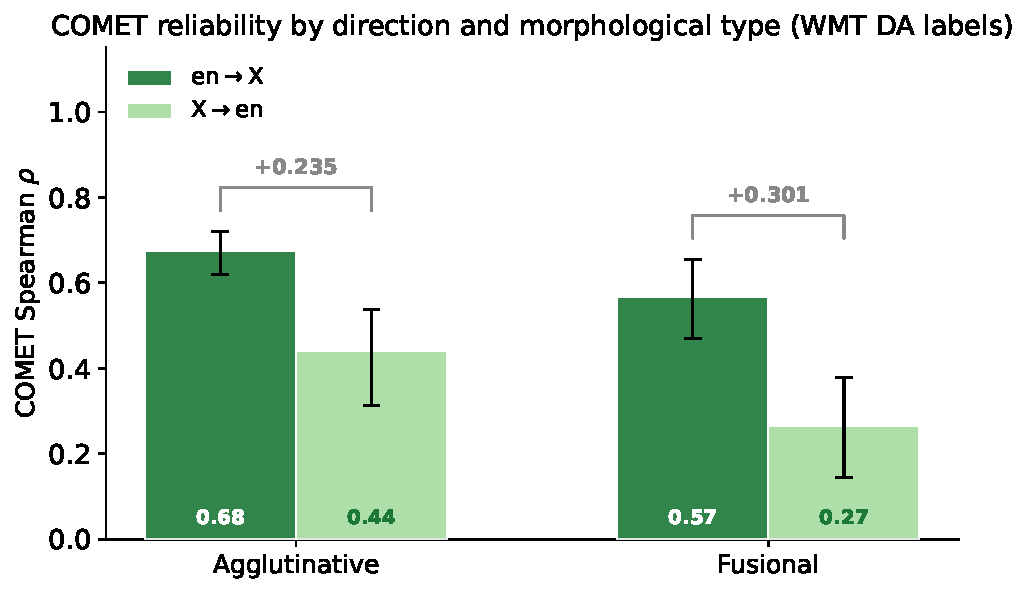
\includegraphics[width=\columnwidth]{figures/presentation_direction_morphology_teaser.pdf}
  \caption{Under WMT DA labels, COMET correlates better with human judgment for en$\to$X (dark green) than for X$\to$en (light green) within both morphological types that have Tier-1 data in both directions (\S\ref{sec:dir_morph}). This direction effect does not replicate consistently under expert MQM labels (\S\ref{sec:mqm_control}). Isolating is omitted because the main pipeline has no en$\to$X isolating pair (en$\to$zh DA exists but was excluded by a configuration rule; see Limitations).}
  \label{fig:teaser}
\end{figure}

Automated MT metrics are the connective tissue of modern MT research: they drive model selection, benchmark comparisons, and shared-task rankings across hundreds of language pairs. Yet the conditions under which these metrics are trustworthy remain poorly understood. A practitioner evaluating a new Hindi or Swahili translation system reaches for BLEU or COMET without knowing whether those metrics bear any reliable relationship to human judgment for that language, domain, or translation direction.

The WMT Metrics Shared Task \cite{freitag2023results} has produced annual meta-evaluations for over a decade, but each edition covers only the language pairs in that year's shared task, typically 5--15 pairs, nearly always news-domain, and never with a systematic typological framing. Efforts to extend coverage to low-resource languages \cite{yari2025item} remain limited in scope. No prior work has unified professional Multidimensional Quality Metrics (MQM) annotations, crowd-sourced Direct Assessment (DA), and synthetic annotations across a common evaluation framework spanning the full range of typological diversity.

We fill this gap with AmanaMT\footnote{\emph{Amana} (Hausa, borrowed from Arabic \emph{am\=ana}): trust, reliability, honesty. Named for the benchmark's purpose: determining when and where automatic MT metrics can be trusted. Code and data: \url{https://github.com/byu-matrix-lab/amana-mt}.}, a unified three-tier benchmark across \NumLanguages\ languages, \NumMetrics\ metrics, and \TotalSegments\ segments. Our design compares metric reliability across resource tiers, translation directions, and morphological types in a single study. The main lesson is about the human labels: several patterns that look like properties of languages or translation directions trace instead to the annotation protocol, to how labels are pooled across years, or to how they were assembled.

\subsection{Contributions}

\textbf{Direction under DA, but not consistently under MQM.} Across a grid of translation direction (en$\to$X, X$\to$en, X$\leftrightarrow$Y) and morphological type (isolating, agglutinative, fusional), direction is the largest predictor of metric--human correlation under WMT DA labels ($\eta^2_{\text{dir}}=\EtaSqDir$, against $\eta^2_{\text{morph}}=\EtaSqMorph$). On segments that also have expert MQM labels, the into-English deficit reverses sign in \MqmCtrlNNegMQM\ of \MqmCtrlNYearsMQM\ WMT years (\S\ref{sec:mqm_control}), so the effect is better explained by into-English crowd DA than by direction itself.

\textbf{Label assembly changes conclusions.} Correcting how we assembled the MQM labels moved per-language correlations substantially (e.g.\ Russian COMET $\rho=\LangCOMETRU$, Spanish $\LangCOMETES$) and reversed several claims of the original version (Version note). We describe the errors so that others building on the same public files can avoid them.

\textbf{Pooling across years can mask failure.} Czech cs-en pooled across WMT years ($\rho=\CsEnPooled$) hides per-year correlations ranging from $\CsEnRangeLo$ to $\CsEnRangeHi$.

\textbf{Neural metrics dominate.} MetricX-24, xCOMET, and COMET outperform surface metrics in every direction and tier, and MetricX-24 has the highest mean correlation in every tier. Which neural metric wins a given language pair is less stable (\S\ref{sec:predictor}).

%% ------------------------------------------
\section{Related Work}
\label{sec:related}

\paragraph{WMT Metrics Shared Task.}
The primary venue for systematic MT metric evaluation is the annual WMT Metrics Shared Task, which has evolved from BLEU-focused comparisons \cite{bojar2017wmt} to MQM-based meta-evaluation \cite{freitag2023results}. Each edition covers 5--15 language pairs with professional MQM annotations, generating yearly rankings. Our work differs in three ways: (1) we aggregate across years rather than evaluating a single shared-task snapshot; (2) we add DA and synthetic annotations for language pairs without MQM; (3) we frame results typologically rather than as a ranking exercise.

\paragraph{MQM and annotation quality.}
\citet{freitag2021experts} establish that expert MQM annotation substantially outperforms crowd-sourced DA for high-quality MT evaluation, and the WMT22 metrics task found segment-level correlations with into-English reference-based crowd DA to be near zero and recommended against using those scores to evaluate metrics \citep[App.~B]{freitag2022results}. \citet{deutsch2023ties} show that tie handling in pairwise accuracy (PA) materially affects rankings; we report a tie-credited PA variant alongside PA (\S\ref{sec:method}). Reference quality as a confound is studied by \citet{freitag2023results}, who argue that ``metrics might be guilty but references are not innocent.''

\paragraph{Metric reliability under domain and resource shift.}
\citet{zouhar2024domain} demonstrate that learned metrics fine-tuned on WMT news data degrade substantially when applied to out-of-domain text. \citet{yari2025item} find that metric reliability varies significantly across Indian languages, with low-resource languages showing systematically weaker correlations, a finding our broader typological framing partially confirms and partially complicates (Khmer is low-resource but correlates well).

\paragraph{Morphology and MT evaluation.}
\citet{mondshine2025ngrams} study metric reliability across morphological types in summarization and find that COMET correlates better for fusional languages, the inverse of the sign we observe within X$\to$en. In MT, morphological type is a much weaker predictor of metric reliability than direction ($\eta^2_{\text{morph}}=\EtaSqMorph$ vs.\ $\eta^2_{\text{dir}}=\EtaSqDir$), an axis absent from monolingual summarization, although that direction effect itself depends on the labels used (\S\ref{sec:mqm_control}). \citet{bugliarello2020xmi} show that MT difficulty (cross-mutual information) is asymmetric across translation direction; we find an asymmetry in metric reliability under DA labels, but not consistently under MQM.

\paragraph{Typological diversity in NLP.}
The broader context for this work is the recognition that NLP systems, including evaluation metrics, are not language-agnostic \cite{costa2022no}. The morphological and directional effects we quantify are one instance of a general pattern: models trained predominantly on English-centric data inherit English-centric assumptions about what good translation looks like.

%% ------------------------------------------
\section{Methodology}
\label{sec:method}

\subsection{Three-Tier Annotation Design}

A core contribution is the unified three-tier data pipeline that brings together human and synthetic annotations under a shared evaluation framework:

\textbf{Tier~1a, WMT MQM} (\textit{high-resource}): Professional Multidimensional Quality Metrics span-level annotations from the WMT shared task \cite{freitag2021experts}, covering en-de, en-ru and zh-en (WMT20--22, from the \texttt{RicardoRei/wmt-mqm-human-evaluation} release) and he-en (WMT23). Segment-level MQM penalty scores are converted to quality scores with the standard weighted formula and then to percentile ranks within each (language, year), because the release stores en-ru WMT21 and WMT22 scores on different scales. he-en (WMT23) and en-es (WMT24) are not in that release; we build them from Google's span-level MQM files, with one row per (system, segment), error markup removed, and canary and reference-as-system rows dropped. The resulting scores agree closely with the official \texttt{mt-metrics-eval} MQM scores. We keep the published tiering, in which en-es is Medium rather than High.

\textbf{Tier~1b, WMT Direct Assessment} (\textit{medium/low-resource}): Sentence-level DA scores from the WMT direct assessment protocol \cite{graham2017crowd} covering cs, tr, uk (medium) and ha, km, ps (low-resource), drawn from the corresponding per-year WMT shared task releases. DA scores are normalized to [0,\,1]. For into-English pairs these are largely reference-based crowd DA, which \citet{freitag2022results} recommend against using at segment level; \S\ref{sec:mqm_control} tests what this does to our direction findings.

\label{sec:tier2}\textbf{Tier~2, Synthetic MQM} (\textit{very-low-resource}): For \NumTierTwoLanguages\ languages with no human MT annotations (sw, ht, lo, th, my, am, ka), we generate hypotheses using NLLB-200 \cite{costa2022no} over FLORES+ \cite{goyal2022flores,costa2022no} source sentences (\texttt{openlanguagedata/flores\_plus}, the community-maintained successor to FLORES-101 that also incorporates the FLORES-200 expansion introduced alongside NLLB-200), then prompt the large language model (LLM) Llama-3.1-8B-Instruct \cite{dubey2024llama3} with an MQM-style few-shot template following \citet{kocmi2023gembamqm} to produce synthetic span-level quality judgments. Validation against human annotation (even 200 Error Span Annotation (ESA)-annotated segments per language) would be required to confirm that Tier~2 synthetic scores reflect real translation quality rather than LLM self-consistency.

\subsection{Metrics Evaluated}

\paragraph{Lexical surface metrics.}
\textbf{BLEU} \cite{papineni2002bleu}: $n$-gram precision with brevity penalty.
\textbf{ChrF++} \cite{popovic2015chrf}: Character $n$-gram F-score with added word-unigram/bigram terms (\texttt{sacrebleu} \texttt{word\_order=2}, the chrF++ configuration); more morphology-sensitive than BLEU.

\paragraph{Embedding-based.}
\textbf{BERTScore} \cite{zhang2019bertscore}: Contextual embedding cosine similarity (mDeBERTa-v3-base).
\textbf{BLEURT} \cite{sellam2020bleurt}: Fine-tuned BERT regression on human ratings. We use \texttt{Elron/bleurt-large-512}, a port of the original English BLEURT-large, and therefore report BLEURT only for English-target segments.

\paragraph{Learned regression (reference-based).}
\textbf{COMET} \cite{rei2022comet22}: Regression over source+hypothesis+reference (wmt22-comet-da).
\textbf{xCOMET} \cite{guerreiro2023xcomet}: COMET with MQM error-span detection (XCOMET-XL).
\textbf{MetricX-24} \cite{juraska2024metricx}: Google's WMT 2024 winning hybrid metric (metricx-24-hybrid-large-v2p6-bfloat16).

\paragraph{Reference-free quality estimation.}
\textbf{CometKiwi-22} \cite{rei2022cometkiwi} (Kiwi-22 in tables): Reference-free QE using source+hypothesis only (wmt22-cometkiwi-da).
\textbf{CometKiwi-23} \cite{rei2023scaling}: Larger 2023 variant (wmt23-cometkiwi-da-xl).

\noindent\textbf{Ensemble}: Min-max normalized score average over the five neural metrics (COMET, xCOMET, MetricX-24, Kiwi-22, Kiwi-23), excluded from Tier~2.

\subsection{Translation Direction and Morphological Type Analysis}
\label{sec:dir_morph}

A central novel contribution is a 2$\times$3 cell analysis of \emph{translation direction} crossed with \emph{morphological type}, defined at the language level as follows.

\vspace{0.3em}
\noindent\textbf{Translation direction:}
\begin{description}[noitemsep,topsep=2pt]
  \item[X$\to$en] non-English source, English target (e.g.\ zh, he, uk)
  \item[en$\to$X] English source, non-English target (e.g.\ de, tr, sw)
  \item[X$\leftrightarrow$Y] neither source nor target is English; each pair is labeled by its target language (e.g.\ fr for de$\to$fr, bn for hi$\to$bn, hi for bn$\to$hi)
\end{description}
Direction is assigned from each segment's language-pair code. \NumMixedLangs\ languages have DA data in both directions; for the direction analyses we split them by direction. Note that for X$\to$en pairs the hypotheses and references are English, so any script or morphology effect there is a property of the source side.
\vspace{0.3em}
\noindent\textbf{Morphological type} (standard linguistic taxonomy):
\begin{description}[noitemsep,topsep=2pt]
  \item[isolating] minimal inflection, meaning via word order (zh, th, lo, km, my)
  \item[agglutinative] transparent suffix/prefix stacking (tr, fi, et, ka, kk, sw, ja, ta, am)
  \item[fusional] multiple grammatical features fused per morpheme (de, ru, es, cs, fr, pl, uk, he, ps, bn, hi, gu, and others)
\end{description}
\vspace{0.3em}

Khmer (km) is Austroasiatic/Mon-Khmer and isolating, not agglutinative as sometimes assumed; Burmese (my) is predominantly analytic. Hausa (ha) is classified fusional here: although it has real agglutinative affixation, its Afroasiatic verbal-grade system fuses aspect, transitivity, and direction via tone and vowel apophony rather than discrete morphemes, and its typology is genuinely mixed rather than a clean fit to either category.

For each language we compute Spearman $\rho$ between each metric and human scores, yielding a matrix of mean $\rho$ per (direction, morphology) cell, with 95\% bootstrap CIs over the languages in each cell. Effect sizes are reported as $\eta^2$ (proportion of variance explained) over the \EtaSqNUnits\ en$\to$X and X$\to$en language--direction units. $\eta^2_{\text{dir}}$ and $\eta^2_{\text{morph}}$ are computed via one-way ANOVA on the per-unit $\rho$ values with direction and morphological type as the respective factors. $\eta^2_{\text{cell}}$ is computed via one-way ANOVA over the \EtaSqNCells\ occupied direction$\times$morphology cells and therefore measures total between-cell variance rather than a formally partitioned interaction term; it is bounded below by each main effect by construction. The informative comparison is therefore how direction dominates the main-effect decomposition ($\eta^2_{\text{dir}}$ much larger than $\eta^2_{\text{morph}}$), while the cell structure ($\eta^2_{\text{cell}}$) captures additional direction-specific morphological variation not visible in either main effect alone.

This analysis is motivated by and extends \citet{mondshine2025ngrams}, who study metric reliability across morphological types in summarization (not MT) and find that COMET correlates \emph{better} for fusional languages in their setting, treating morphology as an independent main driver. In our MT setting morphology is a much weaker predictor than direction ($\eta^2_{\text{morph}}=\EtaSqMorph$, versus $\eta^2_{\text{dir}}=\EtaSqDir$). The direction axis is independently motivated by \citet{bugliarello2020xmi}, who show that translation \emph{difficulty} (measured via cross-mutual information) is asymmetric across direction; we test whether metric \emph{reliability} shows the same asymmetry, and find that the answer depends on the human labels (\S\ref{sec:mqm_control}).

\subsection{Evaluation Protocol}

For each (language, metric) pair, we compute:
(1) Spearman $\rho$ with 95\% bootstrap confidence intervals (1000 resamples, percentile method), resampling source sentences with all of their system outputs together, since outputs of the same source are not independent;
(2) Kendall $\tau$;
(3) Pairwise accuracy (PA), fraction of concordant segment pairs, excluding metric-tied and human-tied pairs \cite{freitag2023results};
(4) Tie-credited pairwise accuracy (\PAhalf{}), which counts metric-tied pairs as one half rather than excluding them, in the spirit of the tie handling of \citet{deutsch2023ties}. This is a segment-level statistic; it is not the system-level soft pairwise accuracy of \citet{thompson2024spa}, and the original version mislabelled it as such;
(5) the Williams test \citep{williams1959,graham2014testing} for the difference between two dependent correlations sharing the human scores, computed on Spearman correlations with $n-3$ degrees of freedom.

Segments where the human quality score is tied are excluded from both PA and \PAhalf{} denominators, following \citet{deutsch2023ties}.

All main analysis runs over \TierOneTotalSegments\ professionally annotated segments across Tier~1a and Tier~1b; the \TotalSegments\ total segment count includes Tier~2 synthetic annotations, which are reported separately and flagged as exploratory.

%% ------------------------------------------
\section{Results and Analysis}
\label{sec:results}

\subsection{Main Correlation Results}

Table~\ref{tab:tier} reports per-tier Spearman $\rho$ and tie-credited pairwise accuracy (\PAhalf{}) averaged across all languages in each tier. Neural regression metrics dominate at every resource level, and MetricX-24 has the highest mean on both measures in every tier. Because each tier uses a different annotation protocol, test sets, and years, these columns are descriptive rather than a test of resource level (Limitations). Williams tests (COMET vs.\ BLEU and vs.\ chrF, per language) confirm COMET's advantage over surface metrics is statistically significant at every Tier~1 language (Tier~1a and Tier~1b) except \WilliamsTierOneExceptionLangs: Ukrainian is discussed below; COMET's own correlation there is near zero, so it cannot significantly exceed anything; Zulu's COMET advantage is significant against BLEU ($p=\WilliamsZUBLEUvsCOMETPval$) but not against chrF ($p=\WilliamsZUCHRFvsCOMETPval$).

Tier~2 synthetic correlations are near-zero across all metrics, most consistent with the local LLM judge (Llama-3.1-8B) failing to produce reliable quality judgments for these low-resource, largely non-Latin-script languages, rather than with the MT metrics themselves failing. This uniform near-zero pattern does not itself distinguish which metric is more reliable for these languages, and we draw no such conclusion from it; without human validation of the synthetic judgments, we cannot separate this LLM-judge-unreliability explanation from a genuine ceiling on metric reliability at this resource level.

We explicitly ruled out a data-pipeline explanation: Tier~2's segment identifiers are shared across all \NumTierTwoLanguages\ languages (each keyed only by FLORES+ sentence index, with no per-language disambiguator), a structurally identical risk to the reference/segment-ID pipeline error affecting the he-en and en-es span-fallback pairs, discussed below (\S\ref{sec:per_lang}) and in Limitations. Independently rebuilding each language's quality scores from the raw synthetic-annotation cache and rejoining by language and segment confirms the reported Tier~2 correlations are correctly aligned, not an artifact of cross-language score bleed. We report Tier~2 for completeness, not as evidence for any typological claim.

\begin{table}[h]
\centering
\small
\setlength{\tabcolsep}{3pt}
\begin{tabular}{llccc}
\toprule
\textbf{Family} & \textbf{Metric} & \textbf{High} & \textbf{Med} & \textbf{Low} \\
 & & \multicolumn{3}{c}{\textit{Spearman $\rho$ / \PAhalf{}}} \\
\midrule
\multirow{2}{*}{Lexical}
  & BLEU       & \TierBLEUHighRho{} / \TierBLEUHighSPA & \TierBLEUMedRho{} / \TierBLEUMedSPA & \TierBLEULowRho{} / \TierBLEULowSPA \\
  & ChrF       & \TierChrFHighRho{} / \TierChrFHighSPA & \TierChrFMedRho{} / \TierChrFMedSPA & \TierChrFLowRho{} / \TierChrFLowSPA \\
\midrule
\multirow{2}{*}{Embed.}
  & BERTScore  & \TierBERTScoreHighRho{} / \TierBERTScoreHighSPA & \TierBERTScoreMedRho{} / \TierBERTScoreMedSPA & \TierBERTScoreLowRho{} / \TierBERTScoreLowSPA \\
  & BLEURT     & \TierBLEURTHighRho{} / \TierBLEURTHighSPA & \TierBLEURTMedRho{} / \TierBLEURTMedSPA & \TierBLEURTLowRho{} / \TierBLEURTLowSPA \\
\midrule
\multirow{3}{*}{Regr.}
  & COMET      & \TierCOMETHighRho{} / \TierCOMETHighSPA & \TierCOMETMedRho{} / \TierCOMETMedSPA & \TierCOMETLowRho{} / \TierCOMETLowSPA \\
  & xCOMET     & \TierxCOMETHighRho{} / \TierxCOMETHighSPA & \TierxCOMETMedRho{} / \TierxCOMETMedSPA & \TierxCOMETLowRho{} / \TierxCOMETLowSPA \\
  & MetricX-24 & \textbf{\TierMetricXHighRho} / \textbf{\TierMetricXHighSPA} & \textbf{\TierMetricXMedRho} / \textbf{\TierMetricXMedSPA} & \textbf{\TierMetricXLowRho} / \textbf{\TierMetricXLowSPA} \\
\midrule
\multirow{2}{*}{QE}
  & Kiwi-22    & \TierKiwiXXIIHighRho{} / \TierKiwiXXIIHighSPA & \TierKiwiXXIIMedRho{} / \TierKiwiXXIIMedSPA & \TierKiwiXXIILowRho{} / \TierKiwiXXIILowSPA \\
  & Kiwi-23    & \TierKiwiXXIIIHighRho{} / \TierKiwiXXIIIHighSPA & \TierKiwiXXIIIMedRho{} / \TierKiwiXXIIIMedSPA & \TierKiwiXXIIILowRho{} / \TierKiwiXXIIILowSPA \\
\midrule
--  & Ensemble & \TierEnsembleHighRho{} / \TierEnsembleHighSPA & \TierEnsembleMedRho{} / \TierEnsembleMedSPA & \TierEnsembleLowRho{} / \TierEnsembleLowSPA \\
\bottomrule
\end{tabular}
\caption{Average Spearman $\rho$ / tie-credited pairwise accuracy (\PAhalf{}) by resource tier. High = Tier~1a MQM (de, ru, zh, he); Med = Tier~1b DA plus en-es WMT24 MQM; Low = Tier~1b DA. Values are averaged across annotation tiers within each resource tier. BLEURT is computed on English-target segments only. \textbf{Bold}: best single metric per tier. Resource tier is confounded with annotation protocol, test set and year (Limitations), so differences between columns should not be read as effects of resource level.}
\label{tab:tier}
\end{table}

\subsection{Per-Language Analysis}
\label{sec:per_lang}

Figure~\ref{fig:heatmap} shows per-language Spearman $\rho$ for COMET. Notable patterns:

\begin{figure*}[t]
  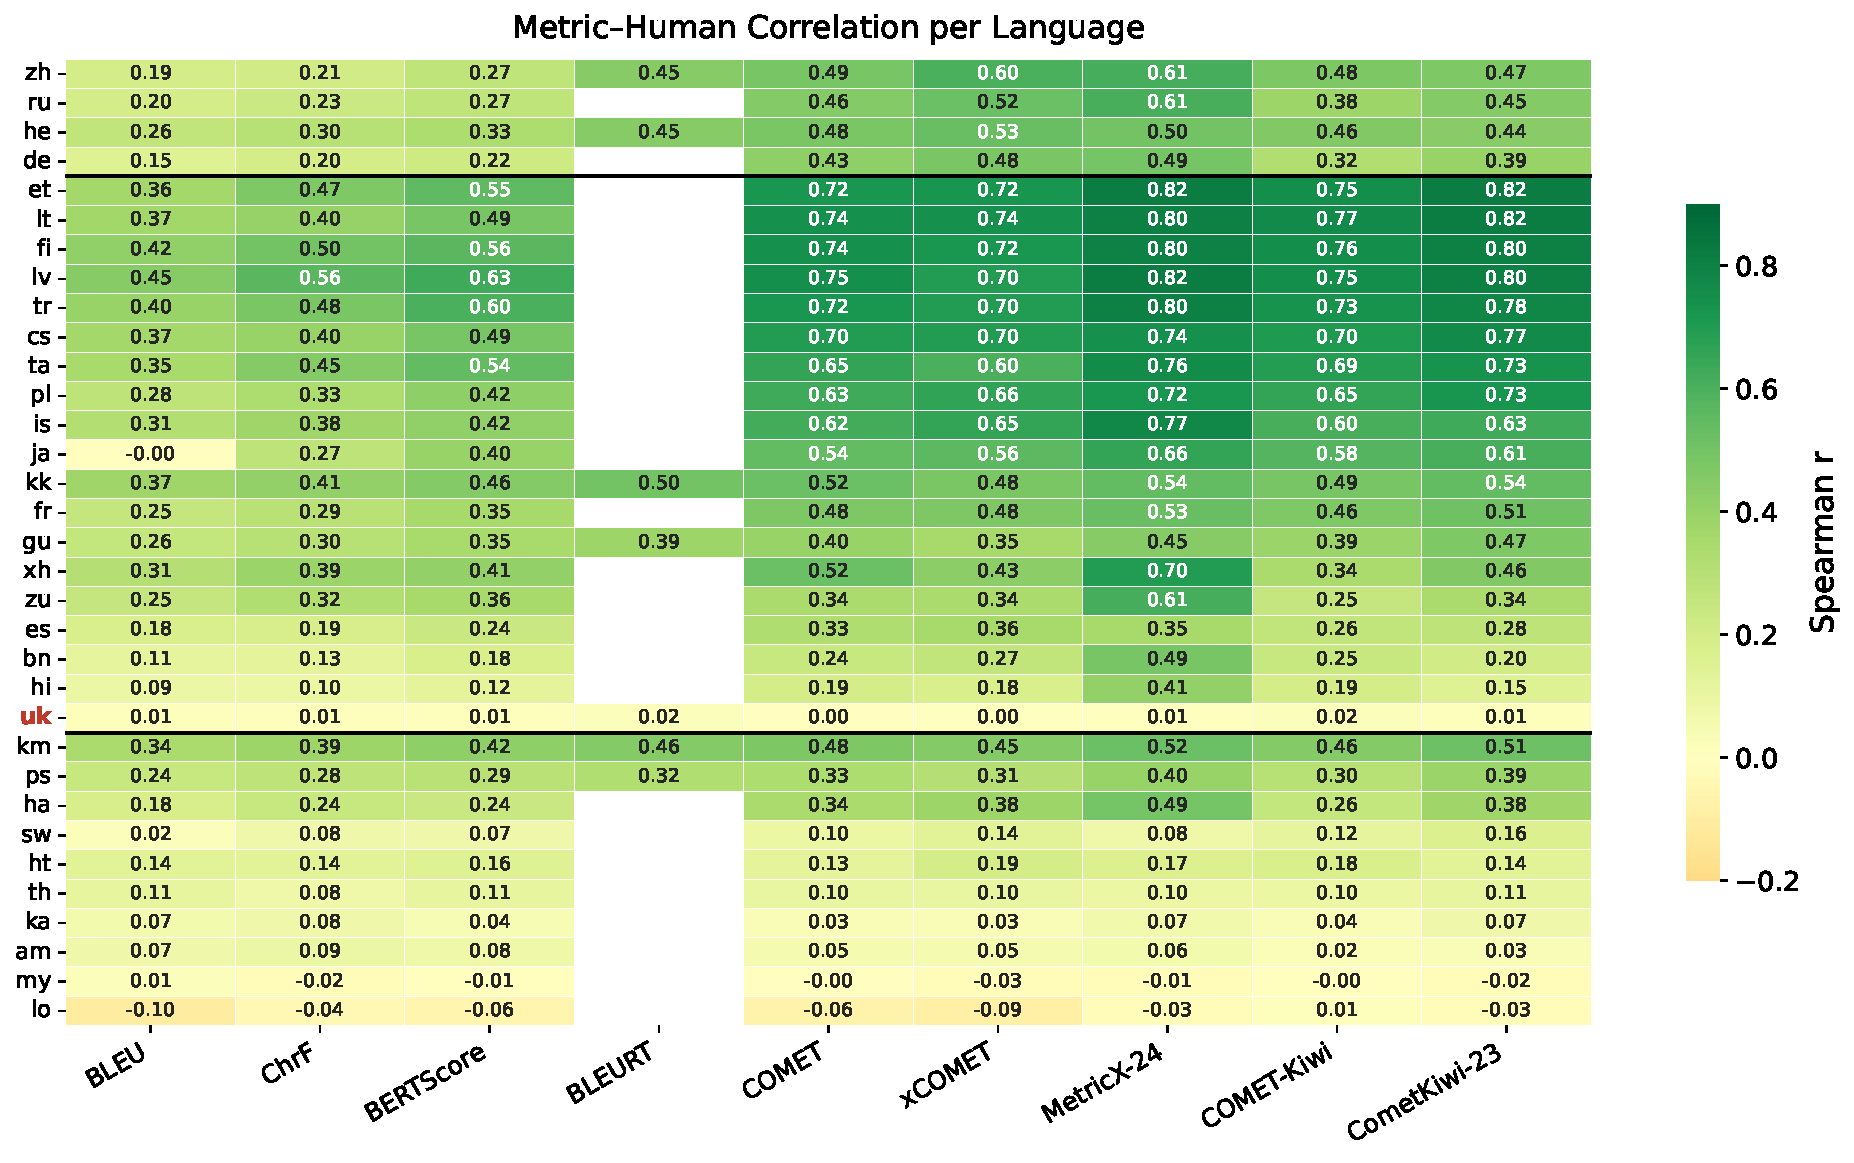
\includegraphics[width=\textwidth]{figures/presentation_language_heatmap.pdf}
  \caption{Per-language Spearman $\rho$ heatmap for all evaluated metrics. Languages sorted by resource tier. Black horizontal lines divide tiers. Ukrainian (\textbf{\textcolor{red!60!black}{uk}}) is near zero for every metric (\S\ref{sec:per_lang}). \textit{Tier~2 languages} (am, ht, ka, lo, my, sw, th) use synthetic MQM annotations generated by Llama-3.1-8B; their correlations are exploratory and unvalidated against human judgments. BLEURT is blank for languages with no English-target segments.}
  \label{fig:heatmap}
\end{figure*}

\textbf{Top performers}: Latvian achieves the highest individual COMET correlation ($\rho = \LangCOMETLV$), followed by Lithuanian ($\SepCOMETLTEX$), Finnish ($\SepCOMETFIEX$), Turkish ($\SepCOMETTREX$), and Estonian ($\SepCOMETETEX$) -- all en$\to$X-specific values for the languages with data in both directions (Table~\ref{tab:dir_sep}), not the direction-pooled averages, which would understate them -- spanning two morphological types. All five are en$\to$X pairs, so their high correlations are part of the direction pattern examined in \S\ref{sec:mqm_control}, not evidence about these languages as such.

\textbf{Ukrainian} (uk-en, WMT22) collapses to near-zero correlation for all metrics ($\rho_{\text{COMET}} = \LangCOMETUK$, pairwise acc.\ $= \LangUKCOMETPairwiseAcc$). A uniform near-zero result across unrelated metric families is also the signature of a broken human-score join, so we independently rebuilt Ukrainian's quality scores from the raw WMT DA data and rejoined them to every metric checkpoint by segment ID: the alignment is correct. The original version attributed the collapse to domain, because every Ukrainian segment carries the domain label \texttt{other}. That explanation does not hold up. The same collapse appears for another WMT22 into-English pair under the same kind of label: on \MqmCtrlZhTwentyTwoN\ WMT22 zh-en segments, COMET correlates at $\rho=\MqmCtrlZhTwentyTwoCOMETCrowdDA$ with the crowd reference-based DA scores but at $\rho=\MqmCtrlZhTwentyTwoCOMETMQM$ with expert MQM and $\rho=\MqmCtrlZhTwentyTwoCOMETSrcDA$ with source-based DA. The likelier cause is therefore the label: WMT22 into-English crowd reference-based DA, which \citet{freitag2022results} found to be uninformative at segment level. We applied the same rebuild-and-rejoin check to is-en and ha-en, the two other pairs with weak correlations (Table~\ref{tab:dir_sep}); both alignments are correct, and both are also into-English crowd DA.

\textbf{Resource tiers.} For every neural metric, the High tier has the higher mean correlation (COMET: $\rho=\TierCOMETHighRho$ vs.\ Medium $\TierCOMETMedRho$; MetricX: $\TierMetricXHighRho$ vs.\ $\TierMetricXMedRho$; Figure~\ref{fig:tierbar}), while BLEU, ChrF++ and BERTScore are slightly higher in Medium. The High--Medium margin for neural metrics depends on how the tier mean is formed: these means average over annotation tiers, so Spanish, the only Medium MQM language, weighs as much as all Medium DA languages together, and averaging over languages instead narrows the margin to near zero. The original version reported the reverse ordering for all metrics and explained it by cross-year pooling; that result came from the MQM label errors corrected in this version. Because the tiers also differ in annotation protocol, test sets and years, we draw no conclusion about resource level from these means.

\textbf{Russian}: pooled COMET $\rho=\LangCOMETRU$ lies between its per-year values (WMT21: $\rho=\RuWmtOneRho$, $n=\RuWmtOneN$; WMT22: $\rho=\RuWmtTwoRho$, $n=\RuWmtTwoN$), so pooling the two years does not suppress it. The original version reported a pooled value far below both years and called it Simpson's paradox. That pooled value was an artifact of normalizing WMT21 and WMT22 en-ru MQM scores together although the two years use different score scales; with scores normalized within each year, the paradox disappears. German behaves the same way (2020: $\rho=\DeWmtTwoZeroRho$; 2021: $\DeWmtTwoOneRho$; 2022: $\DeWmtTwoTwoRho$; pooled: $\LangCOMETDE$).

\textbf{Khmer}: Despite being classified as low-resource, Khmer achieves COMET $\rho=\LangCOMETKM$ and MetricX $\rho=\LangMetricXKM$, higher than several medium-tier languages (e.g., Japanese $\LangCOMETJA$, Hindi $\LangCOMETHI$). Khmer is Austroasiatic (Mon-Khmer) and typologically \emph{isolating}. Its data are a single year of X$\to$en Wikipedia-domain DA; we do not test why it correlates well, and a single test set is weak evidence about the language.

\textbf{Hebrew} (he-en, WMT23 MQM, \LangNHE\ segments): xCOMET has the strongest correlation ($\rho=\LangXCOMETHE$), followed by MetricX ($\LangMetricXHE$), COMET ($\LangCOMETHE$), CometKiwi-22 ($\LangKiwiHE$), CometKiwi-23 ($\LangKiwiXXIIIHE$), and BERTScore ($\LangBERTScoreHE$). Because he-en is into English, the hypotheses are English; Hebrew enters only through the source. The he-en and en-es labels and hypotheses come from Google's span-level MQM files, which the original version parsed incorrectly: error-span markup was left inside the hypotheses, and each error annotation became its own row. Because the markup appears only in hypotheses that contain errors, it gives metrics a signal correlated with the labels, which can inflate correlations; both languages' correlations fell after the correction. We validated the corrected metric scores at segment level against the official \texttt{mt-metrics-eval-v2} \citep{freitag2023results} per-(system, segment) baseline releases for WMT23 he-en and WMT24 en-es, across all \BaselineValNChecks\ (language, metric) checks. COMET and xCOMET, whose checkpoints match the official baselines (\texttt{wmt22-comet-da}, \texttt{XCOMET-XL}), agree closely with the official scores (Pearson/Spearman $r\geq\BaselineValCoreMinPearson$/$\BaselineValCoreMinSpearman$). BLEURT and MetricX agree more weakly (Pearson/Spearman $r\geq\BaselineValMinPearson$/$\BaselineValMinSpearman$), which traces to checkpoint differences rather than alignment: we score BLEURT with an unofficial port of English BLEURT-large rather than \texttt{BLEURT-20}, and the official WMT23 he-en baseline is \texttt{MetricX-23} while we use \texttt{MetricX-24}.

\begin{figure*}[t]
  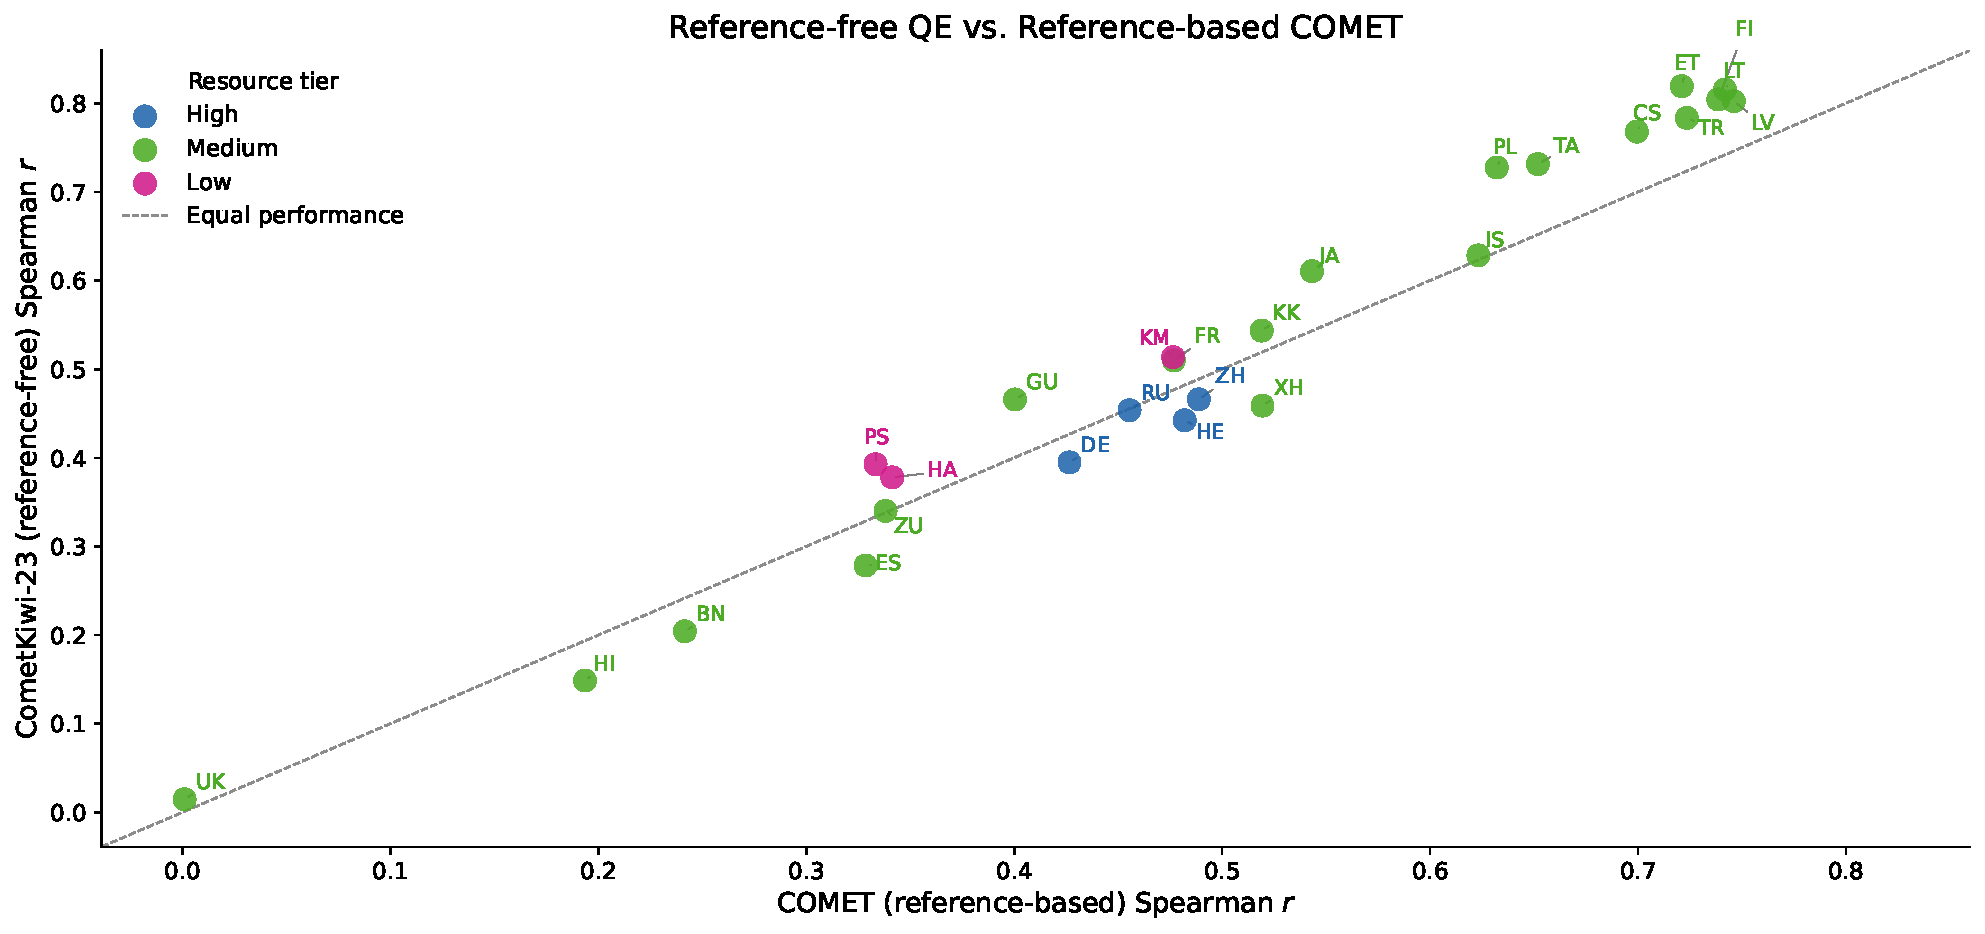
\includegraphics[width=\textwidth]{figures/presentation_kiwi23_vs_comet.pdf}
  \caption{CometKiwi-23 (reference-free) vs.\ COMET (reference-based) Spearman $\rho$ for all \NumHumanAnnotatedLanguages\ languages with human annotations. Most languages lie near the equal-performance diagonal. uk is near zero for both metrics (\S\ref{sec:per_lang}).}
  \label{fig:kiwi_scatter}
\end{figure*}

\textbf{Spanish} (en-es, WMT24 MQM) has the weakest COMET and MetricX correlations of the five MQM languages (MetricX $\rho=\LangMetricXES$, COMET $\rho=\LangCOMETES$). The original version reported it as the strongest; that result came from the parsing errors described above.

\begin{figure*}[t]
  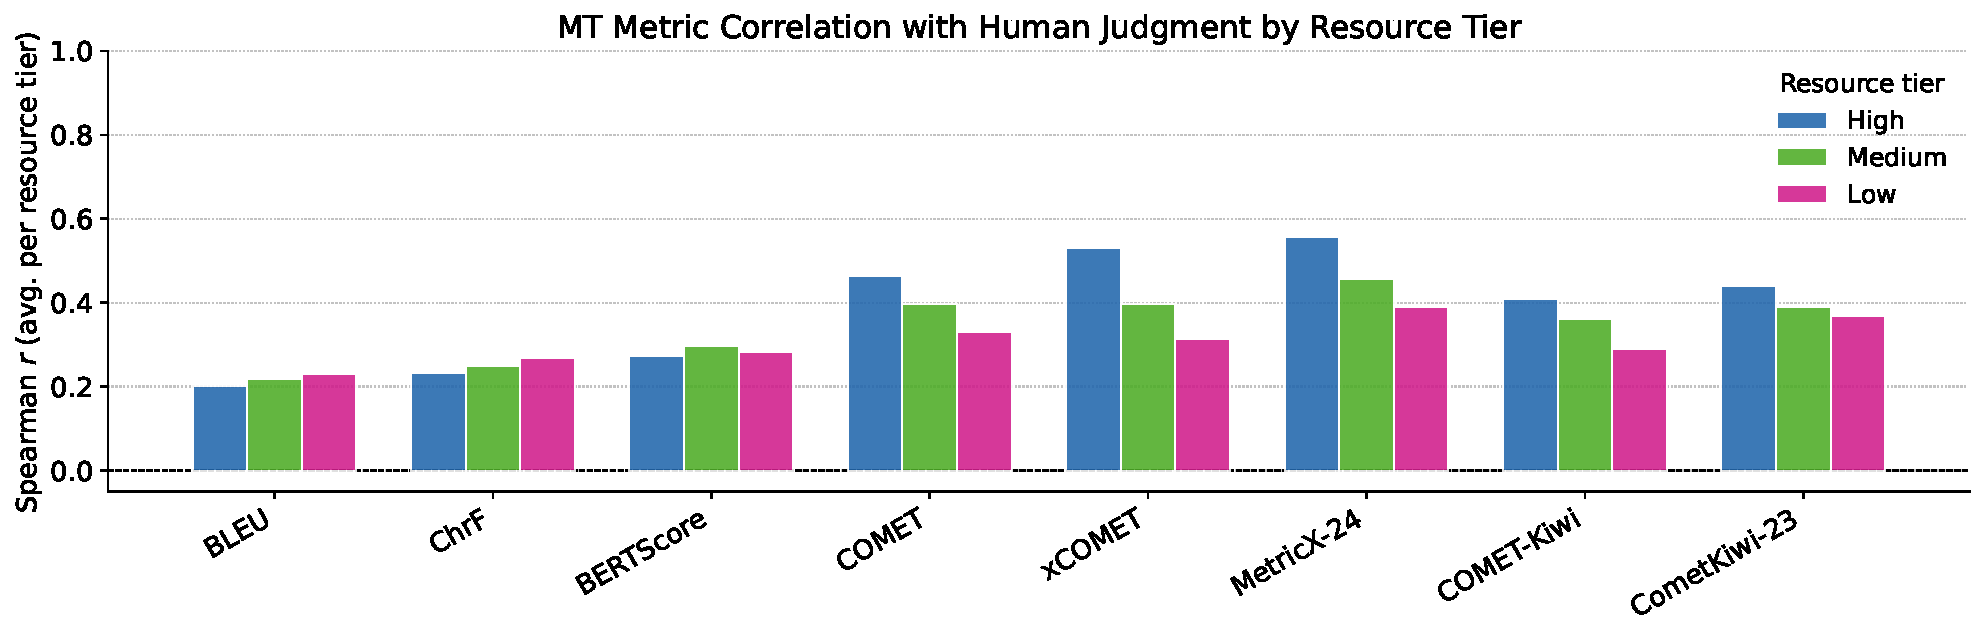
\includegraphics[width=\textwidth]{figures/presentation_tier_bar.pdf}
  \caption{Average Spearman $\rho$ by metric and resource tier. Neural metrics are higher in the High tier than in Medium; the tiers differ in annotation protocol as well as resource level, so the comparison is descriptive (Limitations).}
  \label{fig:tierbar}
\end{figure*}

\subsection{Statistical Robustness}

Bootstrap 95\% CIs, which resample source sentences, are narrower for large test sets (de COMET: $[\LangCOMETDECIlo, \LangCOMETDECIhi]$, $n=\LangNDE$) than for small ones (ps COMET: $[\LangCOMETPSCIlo, \LangCOMETPSCIhi]$, $n=\LangNPS$). All Tier~1a and Tier~1b COMET correlations except Ukrainian are significant at $p < 10^{-10}$ or better; Ukrainian COMET $p = \LangUKCOMETPval$. With test sets this large, statistical significance says little about practical reliability.

\subsection{Translation Direction $\times$ Morphological Type}

Table~\ref{tab:dir_morph} reports the cell means for COMET under the benchmark's labels, which are DA for every pair except the MQM languages (full results for all \NumMetrics\ metrics are in the released code and data repository). \NumMixedLangs\ languages contribute data in both translation directions; we separate them by language-pair code before computing cell means (per-language breakdowns in Table~\ref{tab:dir_sep}). The dominant pattern is directional: en$\to$X languages score substantially above X$\to$en across both morphological types.
\begin{itemize}
  \item \textbf{Agglutinative:} en$\to$X $\rho=\DirMorphCOMETEntoXAgglutin$ vs.\ X$\to$en $\rho=\DirMorphCOMETXtoEnAgglutin$, a gap of $+\GapDirAgglutin$.
  \item \textbf{Fusional:} en$\to$X $\rho=\DirMorphCOMETEntoXFusional$ vs.\ X$\to$en $\rho=\DirMorphCOMETXtoEnFusional$ (depressed by Ukrainian, included here rather than excluded), a gap of $+\GapDirFusional$.
\end{itemize}
The difference-in-differences between the fusional direction gap and the agglutinative direction gap is $\DiDValue$ (Table~\ref{tab:dir_morph}), indicating the direction gap is broadly similar across morphological types. MetricX-24 has the highest mean correlation in every direction (Table~\ref{tab:dir_metric}); which metric wins individual pairs is examined in \S\ref{sec:predictor}.

\paragraph{Robustness: mixed-effects model.} The one-way ANOVAs above treat every (language, direction) row as independent, but \NumMixedLangs\ languages contribute two correlated rows each (one per direction). We therefore also fit a linear mixed-effects model via restricted maximum likelihood (REML): $\rho \sim$ direction + morphology, random intercept per language, $n=\MixedModelNObs$ observations, $\MixedModelNLangs$ languages. Direction is highly significant (X$\to$en coefficient $\MixedModelDirXtoEnCoef$, $p=\MixedModelDirXtoEnP$). The fusional-vs-agglutinative coefficient is smaller but also significant ($\MixedModelMorphFusionalCoef$, $p=\MixedModelMorphFusionalP$); the original version reported it as non-significant. The language random intercept absorbs $\MixedModelICC$ of total variance (the intraclass correlation, ICC). Both terms are detectable once the repeated-measures structure is modeled; direction remains the larger and more robust of the two.

\paragraph{Robustness: year stratification.} Only de, ru, zh, and cs are multi-year in this cell analysis; every other contributing language is single-year. de and ru enter the en$\to$X$\times$fusional cell via their pooled (not year-stratified) $\rho$. Substituting each language's mean of per-year $\rho$ for its pooled value leaves that cell's mean essentially unchanged ($\YearStratEntoXFusionalPooled$ pooled vs.\ $\YearStratEntoXFusionalStrat$ stratified), so year pooling does not explain the en$\to$X advantage. A fully rigorous per-metric training-coverage control (checking whether each metric's training-data volume differs by direction) is not attempted here: none of the \NumMetrics\ metrics publish per-language-pair-and-direction training coverage at the granularity this would require, and we flag it as future work.

\subsection{Does the Direction Effect Survive Expert Labels?}
\label{sec:mqm_control}

The direction effect above rests on DA labels, and for into-English WMT20--22 pairs these are mostly crowd reference-based DA, which \citet[App.~B]{freitag2022results} found to give near-zero, ``completely meaningless'' segment-level correlations for every metric. For \MqmCtrlNPairs\ pairs, WMT also released expert MQM labels (en-de, en-ru, zh-en, he-en), so we can recompute the same-year direction gap (mean en$\to$X minus mean X$\to$en COMET Spearman $\rho$) on the same segment sets under each label type (in WMT23 the MQM gap also includes he-en, which has no DA). This control reads the official \texttt{mt-metrics-eval-v2} files directly, so it does not depend on our data pipeline or on the label corrections in this version. Intervals are 95\% bootstrap CIs resampling source segments.

Under DA the gap is positive in all \MqmCtrlNYearsDA\ years: \MqmCtrlGapDATwenty\ [\MqmCtrlGapDATwentyCIlo, \MqmCtrlGapDATwentyCIhi] in WMT20, \MqmCtrlGapDATwentyOne\ [\MqmCtrlGapDATwentyOneCIlo, \MqmCtrlGapDATwentyOneCIhi] in WMT21, \MqmCtrlGapDATwentyTwo\ [\MqmCtrlGapDATwentyTwoCIlo, \MqmCtrlGapDATwentyTwoCIhi] in WMT22, and \MqmCtrlGapDATwentyThree\ [\MqmCtrlGapDATwentyThreeCIlo, \MqmCtrlGapDATwentyThreeCIhi] in WMT23. Under MQM it is \MqmCtrlGapMQMTwenty\ [\MqmCtrlGapMQMTwentyCIlo, \MqmCtrlGapMQMTwentyCIhi], \MqmCtrlGapMQMTwentyOne\ [\MqmCtrlGapMQMTwentyOneCIlo, \MqmCtrlGapMQMTwentyOneCIhi], \MqmCtrlGapMQMTwentyTwo\ [\MqmCtrlGapMQMTwentyTwoCIlo, \MqmCtrlGapMQMTwentyTwoCIhi], and \MqmCtrlGapMQMTwentyThree\ [\MqmCtrlGapMQMTwentyThreeCIlo, \MqmCtrlGapMQMTwentyThreeCIhi]: X$\to$en is the \emph{better}-evaluated direction in \MqmCtrlNNegMQM\ of \MqmCtrlNYearsMQM\ years. The WMT22 zh-en segments with three label types show where the difference comes from: COMET correlates at $\rho=\MqmCtrlZhTwentyTwoCOMETMQM$ with MQM, $\MqmCtrlZhTwentyTwoCOMETSrcDA$ with source-based DA, and $\MqmCtrlZhTwentyTwoCOMETCrowdDA$ with crowd reference-based DA ($n=\MqmCtrlZhTwentyTwoN$).

We therefore do not claim that translation direction itself predicts metric reliability. The direction effect in Table~\ref{tab:dir_morph} does not replicate consistently under expert MQM, and it is largely explained by into-English crowd DA. This control has limits of its own: only \MqmCtrlNPairs\ pairs have expert labels, so direction is entangled with language; the WMT20--22 sets include human reference translations scored as systems, and excluding them or he-en leaves every sign unchanged in an independent recomputation; and in WMT23, whose DA is source-based, en$\to$X is better evaluated under both label types. A fuller treatment is left to follow-up work.

\begin{table}[t]
\centering
\small
\setlength{\tabcolsep}{3pt}
\begin{tabular}{lccc}
\toprule
\textbf{Dir.} & \textbf{Isol.} & \textbf{Agglutin.} & \textbf{Fusional} \\
 & \multicolumn{3}{c}{\textit{Mean COMET $\rho$ [95\% CI]}} \\
\midrule
X$\to$en  & \DirMorphCOMETXtoEnIsolating{} [---] & \textbf{\DirMorphCOMETXtoEnAgglutin}{\scriptsize[\DirMorphCOMETXtoEnAgglutinCIlo,\DirMorphCOMETXtoEnAgglutinCIhi]} & \DirMorphCOMETXtoEnFusional{}{\scriptsize[\DirMorphCOMETXtoEnFusionalCIlo,\DirMorphCOMETXtoEnFusionalCIhi]} \\
en$\to$X  & --            & \DirMorphCOMETEntoXAgglutin{}{\scriptsize[\DirMorphCOMETEntoXAgglutinCIlo,\DirMorphCOMETEntoXAgglutinCIhi]} & \DirMorphCOMETEntoXFusional{}{\scriptsize[\DirMorphCOMETEntoXFusionalCIlo,\DirMorphCOMETEntoXFusionalCIhi]} \\
X$\leftrightarrow$Y      & --            & --                 & \DirMorphCOMETPivotFusional{}{\scriptsize[\DirMorphCOMETPivotFusionalCIlo,\DirMorphCOMETPivotFusionalCIhi]} \\
\midrule
$\eta^2_{\text{dir}}$ & \multicolumn{3}{c}{\EtaSqDir} \\
$\eta^2_{\text{morph}}$ & \multicolumn{3}{c}{\EtaSqMorph} \\
$\eta^2_{\text{cell}}$ & \multicolumn{3}{c}{\EtaSqCell} \\
\bottomrule
\end{tabular}
\caption{Mean COMET Spearman $\rho$ by translation direction and morphological type, under the benchmark's (mostly DA) labels; see \S\ref{sec:mqm_control} for the same comparison under MQM. Cells with $n{\le}2$ languages have no CI (marked [---]). Empty (--) = no Tier-1 languages in that cell. $\eta^2$ via one-way ANOVA on per-unit $\rho$ over the en$\to$X and X$\to$en units. Russian ($\rho=\LangCOMETRU$, en$\to$X+fusional) and Ukrainian ($\rho=\LangCOMETUK$, X$\to$en+fusional) are included in their cells. \textbf{Bold} marks the X$\to$en agglutinative cell because it is where CometKiwi-23 (not shown in this COMET-only table) wins \WinXtoEnAgglutin\ of \WinTotalXtoEnAgglutin\ direction-separated pairs (Table~\ref{tab:dir_sep}).}
\label{tab:dir_morph}
\end{table}

\begin{table}[h]
\centering
\small
\setlength{\tabcolsep}{1pt}
\begin{tabular}{lccccc}
\toprule
\textbf{Direction} & \textbf{BLEU} & \textbf{ChrF++} & \textbf{COMET} & \textbf{xCOMET} & \textbf{MetricX} \\
\midrule
en$\to$X  & \DirMetricBLEUEntoX & \DirMetricChrFEntoX & \DirMetricCOMETEntoX & \DirMetricxCOMETEntoX & \textbf{\DirMetricMetricXEntoX} \\
X$\to$en  & \DirMetricBLEUXtoEn & \DirMetricChrFXtoEn & \DirMetricCOMETXtoEn & \DirMetricxCOMETXtoEn & \textbf{\DirMetricMetricXXtoEn} \\
X$\leftrightarrow$Y      & \DirMetricBLEUPivot & \DirMetricChrFPivot & \DirMetricCOMETPivot & \DirMetricxCOMETPivot & \textbf{\DirMetricMetricXPivot} \\
\bottomrule
\end{tabular}
\caption{Mean Spearman $\rho$ by translation direction for five representative metrics (averaged across all languages in each direction group). MetricX-24 leads across all three directions among these five metrics, including X$\to$en, where it now edges out CometKiwi-23 (not shown) by a narrow margin ($\rho{=}\DirMetricMetricXXtoEn$ vs.\ $\rho{=}\DirMetricCKXXIIIXtoEn$); this pooled ranking is not the same question as which metric wins the most individual X$\to$en language pairs (Table~\ref{tab:lookup}), where CometKiwi-23 wins more often. X$\leftrightarrow$Y pairs show the lowest surface-metric scores.}
\label{tab:dir_metric}
\end{table}

Contrast with \citet{mondshine2025ngrams}: in their summarization setting, COMET correlates \emph{better} for fusional languages. Under our DA labels, fusional X$\to$en languages score $\rho=\DirMorphCOMETXtoEnFusional$ and fusional en$\to$X languages $\rho=\DirMorphCOMETEntoXFusional$, a gap of $+\GapDirFusional$; agglutinative languages show the same directional pattern ($\rho=\DirMorphCOMETXtoEnAgglutin$ X$\to$en vs.\ $\rho=\DirMorphCOMETEntoXAgglutin$ en$\to$X, a gap of $+\GapDirAgglutin$). Within each direction, agglutinative languages score above fusional ones, and the mixed-effects model detects this morphology term. The empty en$\to$X isolating cell limits what the design can say about isolating languages (Limitations).

\subsection{Typological Predictors of Metric Choice}
\label{sec:predictor}

We now ask a practical question: which metric should a practitioner prefer for an unseen language pair? The analysis in this section is exploratory; cells are small and the labels are those of \S\ref{sec:dir_morph}.

For each of the \NumHumanAnnotatedLanguages\ languages with human annotations, we rank all metrics by Spearman $\rho$ and record the best-performing metric.
Table~\ref{tab:lookup} summarizes these \TableFourTotalPairs\ direction-language pair observations (\TableFourMainPipelinePairs\ in the main pipeline; de-en held out as a blind validation), with leave-one-out (LOO) cross-validation for cells with $n \geq 6$ (overall \LOOOverallCorrect/\LOOOverallTotal\ = \LOOOverallPct\%). Isolating X$\to$en ($n{=}\WinTotalXtoEnIsolating$) and X$\leftrightarrow$Y ($n{=}\PivotN$) fall below this threshold and are marked `--' in the LOO column rather than validated.
The most robust pattern in the table needs no morphological breakdown at all: CometKiwi-23 beats COMET in all \BeatsCometEntoXAgglutin\ of \WinTotalEntoXAgglutin\ agglutinative and \BeatsCometEntoXFusional\ of \WinTotalEntoXFusional\ fusional en$\to$X pairs (\BeatsCometEntoXTotal/\EntoXTotalPairs\ overall), with exact (Clopper--Pearson) 95\% CIs on the win fraction of $[\CellCIEntoXAgglutinLo, \CellCIEntoXAgglutinHi]$ and $[\CellCIEntoXFusionalLo, \CellCIEntoXFusionalHi]$. Table~\ref{tab:lookup} is organized first by direction, the dominant factor, and then by morphological type within each direction as a secondary refinement: even though morphology explains substantially less of the aggregate variance in reliability than direction does ($\eta^2_{\text{morph}}=\EtaSqMorph$ vs.\ $\eta^2_{\text{dir}}=\EtaSqDir$), the within-direction agglutinative-vs-fusional splits are large enough to flip which specific metric wins the discrete argmax comparison (\S\ref{sec:dir_morph}), so morphology remains a useful secondary key for the practitioner-facing recommendation even though it is not the primary driver of reliability.
Three patterns emerge, with decreasing confidence:

\begin{enumerate}[leftmargin=*,itemsep=4pt,topsep=4pt]
  \item \textbf{X$\to$en: CometKiwi-23 usually wins agglutinative pairs; fusional is split.} CometKiwi-23 is the best metric for \WinXtoEnAgglutin/\WinTotalXtoEnAgglutin\ agglutinative X$\to$en pairs (LOO \LOOXtoEnAgglutin/\LOOTotalXtoEnAgglutin; exact CI on CometKiwi-23$>$COMET: $[\CellCIXtoEnAgglutinLo, \CellCIXtoEnAgglutinHi]$) but only \WinXtoEnFusional/\WinTotalXtoEnFusional\ fusional ones (including Hebrew and the held-out de-en; LOO \LOOXtoEnFusional/\LOOTotalXtoEnFusional\ over the DA-pipeline subset; see Table~\ref{tab:lookup}'s note). On the held-out de-en pair ($n{=}\DeEnN$; German otherwise enters the pipeline only as en$\to$de MQM), CometKiwi-23 reaches $\rho{=}\DeEnKiwiRho$ vs.\ MetricX $\rho{=}\DeEnMetricXRho$ and COMET $\rho{=}\DeEnCOMETRho$: CometKiwi-23 wins, but by a small margin.

  \item \textbf{en$\to$X: MetricX usually wins agglutinative pairs; fusional is split.} For agglutinative en$\to$X (\WinTotalEntoXAgglutin{} languages), MetricX wins \WinEntoXAgglutin/\WinTotalEntoXAgglutin{} (LOO \LOOEntoXAgglutin/\LOOTotalEntoXAgglutin), though margins are often small (kk: MetricX $\SepMXKKEX$ vs.\ CometKiwi-23 $\SepCKXXIIIKKEX$; tr: $\SepMXTREX$ vs.\ $\SepCKXXIIITREX$). CometKiwi-23 still beats COMET in \BeatsCometEntoXAgglutin/\WinTotalEntoXAgglutin{} agglutinative en$\to$X pairs (exact CI $[\CellCIEntoXAgglutinLo, \CellCIEntoXAgglutinHi]$), so the choice between CometKiwi-23 and COMET is clear; the MetricX advantage only matters when choosing between all three neural metrics. For fusional en$\to$X (\WinTotalEntoXFusional{} languages), CometKiwi-23 wins \WinEntoXFusional/\WinTotalEntoXFusional{} and MetricX-24 most of the rest; CometKiwi-23 beats COMET in \BeatsCometEntoXFusional/\WinTotalEntoXFusional{} (CI $[\CellCIEntoXFusionalLo, \CellCIEntoXFusionalHi]$).

  \item \textbf{Isolating X$\to$en and X$\leftrightarrow$Y: MetricX.} MetricX-24 wins both isolating X$\to$en cases (zh: $+\GapZHMetricXBleu$ over BLEU; km: $+\GapKMMetricXBleu$; average $+\TableFourXtoEnIsolating$) and all X$\leftrightarrow$Y pairs (\PivotMetricXWins/\PivotN), where neither source nor target is English. Both cells are too small for cross-validation.
\end{enumerate}

Across all profiles, the gain over BLEU from choosing the recommended metric ranges from $+\TableFourXtoEnFusional$ to $+\TableFourEntoXAgglutin$ Spearman $\rho$ (Table~\ref{tab:lookup}), the ``always use a neural metric'' message is robust even where the \emph{choice} among neural metrics is uncertain.

\begin{table*}[t]
\centering
\small
\setlength{\tabcolsep}{6pt}
\begin{tabular}{llcllc}
\toprule
\textbf{Direction} & \textbf{Morphological type} & \textbf{$n$ pairs} & \textbf{Recommended metric} & \textbf{LOO accuracy} & \textbf{Avg $\Delta\rho$ vs.\ BLEU} \\
\midrule
X$\to$en & Agglutinative & \WinTotalXtoEnAgglutin   & CometKiwi-23 (\WinXtoEnAgglutin/\WinTotalXtoEnAgglutin)          & \LOOXtoEnAgglutin/\LOOTotalXtoEnAgglutin & $+\TableFourXtoEnAgglutin$ \\
X$\to$en & Isolating     & \WinTotalXtoEnIsolating   & MetricX-24 (\WinXtoEnIsolating/\WinTotalXtoEnIsolating)            & --  & $+\TableFourXtoEnIsolating$ \\
X$\to$en & Fusional      & \WinTotalXtoEnFusional$^\dagger$ & CometKiwi-23 (\WinXtoEnFusional/\WinTotalXtoEnFusional)   & \LOOXtoEnFusional/\LOOTotalXtoEnFusional & $+\TableFourXtoEnFusional$ \\
en$\to$X & Agglutinative & \WinTotalEntoXAgglutin   & MetricX-24 (\WinEntoXAgglutin/\WinTotalEntoXAgglutin)$^\ddagger$  & \LOOEntoXAgglutin/\LOOTotalEntoXAgglutin & $+\TableFourEntoXAgglutin$ \\
en$\to$X & Fusional      & \WinTotalEntoXFusional   & CometKiwi-23 (\WinEntoXFusional/\WinTotalEntoXFusional)          & \LOOEntoXFusional/\LOOTotalEntoXFusional & $+\TableFourEntoXFusional$ \\
X$\leftrightarrow$Y & Fusional      & \PivotN   & MetricX-24 (\PivotMetricXWins/\PivotN)            & --  & $+\TableFourPivotFusional$ \\
\bottomrule
\end{tabular}
\caption{\textbf{Exploratory metric selection guide}: most frequent best metric among COMET, CometKiwi-23 and MetricX-24 per profile, across \TableFourTotalPairs\ direction--language pair observations (de-en held out), under the benchmark's mostly DA labels. $n$ = number of direction-separated pairs; LOO accuracy = leave-one-out cross-validation (-- = cell too small to validate); Avg $\Delta\rho$ = mean Spearman gain over BLEU. Margins between the top neural metrics are often small. $^\dagger$Fusional X$\to$en's $n{=}\WinTotalXtoEnFusional$ includes Hebrew and the held-out de-en pair, neither scored by the DA direction-separated pipeline the LOO cross-validation runs over; its LOO column therefore covers only \LOOTotalXtoEnFusional\ DA-pipeline languages. Held-out de-en ($n{=}\DeEnN$): CometKiwi-23 $\rho{=}\DeEnKiwiRho$ vs.\ COMET $\rho{=}\DeEnCOMETRho$. $^\ddagger$Agglutinative en$\to$X: MetricX-24 wins \WinEntoXAgglutin/\WinTotalEntoXAgglutin, and CometKiwi-23 beats COMET in \BeatsCometEntoXAgglutin/\WinTotalEntoXAgglutin{} (exact CI $[\CellCIEntoXAgglutinLo,\CellCIEntoXAgglutinHi]$); the MetricX advantage is under $\KkTrMaxMargin$ $\rho$ for kk and tr.}
\label{tab:lookup}
\end{table*}

As a post-hoc check, we trained a Ridge regression predictor (World Atlas of Language Structures \citep[WALS;][]{wals} typological features + morphological type + direction, leave-one-language-out cross-validation (LOLO-CV), $n{=}\RidgeNUnits$ language--direction units from \RidgeNLangs\ Tier-1 languages, with both directions of a language held out together). Pearson $r=\RidgeCKXXIIIPearson$ for CometKiwi-23 and $r=\RidgeCKPearson$ for Kiwi-22; recommendation accuracy is \RidgeRecAcc, too low to treat the predictor as deployable. The moderate $r$ for the CK family confirms that direction and CK advantage are partially co-predictable from typological features, but the low recommendation accuracy is a negative result on the stronger claim that typological features alone suffice to select among neural metrics. Recommendation accuracy counts units.

%% ------------------------------------------
\section{Discussion}
\label{sec:discussion}

\subsection{The Neural-Surface Gap Scales With Morphological Complexity}

This is a claim about a different quantity than \S\ref{sec:dir_morph}: $\eta^2_{\text{morph}}=\EtaSqMorph$ measures how much morphological type explains variance in absolute metric--human correlation, and it is small. The finding here concerns the \emph{gap} between neural and surface metrics, a derived quantity that morphology predicts much more strongly than it predicts either metric's raw reliability. COMET, xCOMET, and MetricX-24 lead at every tier and in every direction (Tables~\ref{tab:tier} and~\ref{tab:dir_metric}), but their gap over surface metrics is not uniform: it is larger for agglutinative languages.

For fusional X$\to$en languages (excluding Ukrainian), the COMET--BLEU gap averages $\GapCometBleuFusionalXtoEn$ Spearman points; holding direction fixed, agglutinative X$\to$en languages show a larger gap still, $\GapCometBleuAgglutinXtoEn$ (the same pattern holds en$\to$X, where the gap is $\GapCometBleuAgglutinEntoX$ for agglutinative languages). This is not simply a ceiling artifact of agglutinative X$\to$en being an easier cell overall: within X$\to$en, BLEU's own reliability is nearly flat across morphological type ($\rho\approx\DirMetricBLEUXtoEn$ pooled; agglutinative and fusional differ by only a few points), while COMET's reliability rises substantially from fusional to agglutinative. The widening gap comes from COMET tracking something morphology-related that BLEU does not, not from BLEU degrading uniformly.

This is consistent with $n$-gram overlap systematically underestimating adequacy when target morphology is rich: a correct translation of a Finnish verb may share zero surface $n$-grams with the reference if a different but equally valid inflected form was chosen. Neural metrics are comparatively insensitive to this effect, which is exactly why morphology moves their reliability much less than it moves direction ($\eta^2_{\text{morph}}=\EtaSqMorph$ vs.\ $\eta^2_{\text{dir}}=\EtaSqDir$) while still moving the size of their advantage over BLEU. This pattern rests on two cells per direction without CIs on the gap itself, under the same DA labels as \S\ref{sec:dir_morph}, and should be read as descriptive.

\subsection{Label Quality Explains the Largest Anomalies}
\label{sec:label_quality}

Every large anomaly in the original version traced to the human labels rather than to a language. Ukrainian's collapse matches the collapse of other WMT22 into-English crowd DA (\S\ref{sec:per_lang}); the direction effect does not replicate consistently under MQM (\S\ref{sec:mqm_control}); Russian's apparent Simpson's paradox came from normalizing two MQM score scales together; and the Hebrew and Spanish results came from parsing errors that let error markup into the hypotheses. Only the last two were our own mistakes, but all four look, at first, like findings about languages or directions. Two practical lessons follow: check a reliability finding against expert labels before attributing it to a language or direction, and check that labels assembled from several releases are on one scale and aligned with the text being scored.

\paragraph{Always stratify by year.}
Table~\ref{tab:yearstrat} compares pooled and year-stratified COMET correlations. With labels normalized within year, pooling barely changes the MQM languages ($\Delta$ near zero), but it can hide heterogeneity: Czech cs-en pooled $\rho=\CsEnPooled$ masks a per-year range of $[\CsEnRangeLo,\ \CsEnRangeHi]$, including metric failure in 2021 and strong correlation in 2017. Per-year results should be reported alongside pooled ones.

\begin{table}[h]
\centering\small
\setlength{\tabcolsep}{2pt}
\begin{tabular}{llcccc}
\toprule
\textbf{Lang} & \textbf{Tier} & \textbf{Years} & \textbf{Pooled $\rho$} & \textbf{Year $\rho$ range} & $\Delta$ \\
\midrule
ru    & MQM & 2021--22   & \LangCOMETRU & $[\RuRangeLo,\ \RuRangeHi]$ & $\RuDelta$ \\
zh    & MQM & 2020--22   & \LangCOMETZH & $[\ZhRangeLo,\ \ZhRangeHi]$ & $\ZhDelta$ \\
de    & MQM & 2020--22   & \LangCOMETDE & $[\DeRangeLo,\ \DeRangeHi]$ & $\DeDelta$ \\
cs-en & DA  & 2017--22   & $\CsEnPooled$ & $[\CsEnRangeLo,\ \CsEnRangeHi]$ & $\CsEnDelta$ \\
\bottomrule
\end{tabular}
\caption{Year-stratified vs.\ pooled COMET Spearman $\rho$ for languages with multiple WMT years. $\Delta$ = stratified mean $-$ pooled. Year $\rho$ range = [$\min$, $\max$] per-year $\rho$. MQM scores are normalized within each year. Czech cs-en (pooled $\CsEnPooled$, year range $[\CsEnRangeLo,\, \CsEnRangeHi]$) shows how pooling masks heterogeneity.}
\label{tab:yearstrat}
\end{table}

%% ------------------------------------------
\section{Conclusion}
\label{sec:conclusion}

We presented a unified meta-evaluation of \NumMetrics\ MT metrics across \NumLanguages\ languages, three annotation tiers, and \TotalSegments\ segments, with the goal of understanding \emph{when} metrics can be trusted and \emph{why} they appear to fail.

The central finding of this corrected version is that the human labels decide much of the answer. Under WMT DA labels, translation direction is the largest predictor of metric reliability ($\eta^2_{\text{dir}}=\EtaSqDir$, against $\eta^2_{\text{morph}}=\EtaSqMorph$), but on segments with expert MQM labels the into-English deficit reverses in \MqmCtrlNNegMQM\ of \MqmCtrlNYearsMQM\ WMT years; it is better explained by into-English crowd reference-based DA than by direction. Ukrainian's collapse fits the same explanation. Errors in how we assembled MQM labels produced the original version's Russian Simpson's paradox, its Medium-over-High tier ordering, and its Hebrew and Spanish results. None of these were findings about languages.

What survives is less surprising but more robust: neural metrics are substantially better than surface metrics in every direction and tier. The en$\to$X gap between MetricX-24 ($\rho\approx\DirMetricMetricXEntoX$) and BLEU ($\rho\approx\DirMetricBLEUEntoX$) is large enough that any evaluation still using BLEU as its primary metric should be revisited.

\paragraph{A practical, exploratory procedure.} Table~\ref{tab:lookup} suggests a short recipe for choosing a metric on an unseen language pair. Margins between the top neural metrics are often small, and the recipe is based on the benchmark's mostly DA labels.
\begin{enumerate}
  \item \textbf{Prefer a neural metric over BLEU/ChrF++.} The gain ranges from $+\TableFourXtoEnFusional$ to $+\TableFourEntoXAgglutin$ Spearman points across the profiles in Table~\ref{tab:lookup}.
  \item \textbf{Among neural metrics, MetricX-24 is the safest default}: it has the highest mean correlation in every tier and direction, and wins every isolating X$\to$en and X$\leftrightarrow$Y pair.
  \item \textbf{CometKiwi-23 is competitive where no reference is available}: it beats COMET in \BeatsCometEntoXTotal/\EntoXTotalPairs\ en$\to$X pairs and wins most agglutinative X$\to$en pairs.
  \item \textbf{Typological features alone will not pick the metric}: our Ridge predictor over WALS \citep{wals} features reaches only \RidgeRecAcc\ recommendation accuracy.
  \item \textbf{Check the labels} before trusting any reliability estimate for a new pair: in particular, avoid segment-level conclusions from into-English crowd reference-based DA \citep{freitag2022results}.
\end{enumerate}

Future work should test the direction question on more pairs with expert labels, compare resource levels with the annotation protocol held fixed, and validate the Tier~2 synthetic annotations against human judgments. Our claims throughout are associational, not causal. A within-language, within-year comparison of MQM and DA on more pairs would separate the annotation-protocol effect from resource level and direction; \S\ref{sec:mqm_control} is a first step on the pairs that allow it.

%% ------------------------------------------
\section*{Limitations}
\label{sec:limitations}

\textbf{Label quality.} Most into-English DA in WMT20--22 is crowd reference-based, which \citet{freitag2022results} recommend against using at segment level; our direction, morphology and metric-selection analyses use these labels for many X$\to$en pairs. The MQM control (\S\ref{sec:mqm_control}) covers only \MqmCtrlNPairs\ pairs. Tier~2 synthetic annotations have not been validated against human judgments; Tier~2 results are exploratory.

\textbf{Label assembly.} The original version of this paper had errors in how MQM labels were assembled (Version note). We now normalize MQM scores within each (language, year), build he-en and en-es from Google's span files with markup removed, and test the result against the official MQM scores. We evaluate he-en and en-es against a single reference (refA) throughout. The MQM data include human reference translations scored as systems (e.g.\ \texttt{Human-A}, \texttt{refB}); we keep them, as the published analysis did.

\textbf{Data excluded by configuration.} A configuration rule skipped WMT DA for de, ru and zh, which were already loaded as MQM, and the language label merges both directions, so the DA data for en-de, en-ru, en-zh, de-en, ru-en and zh-en, and for fr-de, were not used. This includes en$\to$zh, the only en$\to$X isolating pair available. The MQM data also omit some available releases (WMT23 en-de and zh-en, WMT24 en-de). Incorporating them would change the direction$\times$morphology analysis.

\textbf{Empty en$\to$X isolating cell.} Because en$\to$zh was excluded, the main pipeline has no en$\to$X isolating observation, which limits what the design can say about isolating languages.

\textbf{Metric implementations.} BLEURT is an unofficial port of English BLEURT-large, so we report it only for English-target segments. BLEU uses the \texttt{13a} tokenizer, which does not segment Japanese or Chinese, so BLEU is underestimated for en-ja and similar pairs; this narrows but does not remove the neural advantage. Several learned metrics were trained on earlier WMT human judgments, and we did not check every test year against each metric's training data.

\textbf{Pooling.} Per-language correlations pool test sets, years and domains (\S\ref{sec:discussion} reports per-year values for the multi-year languages).

\textbf{Language non-independence in the direction$\times$morphology analysis.} \NumMixedLangs\ languages contribute per-language $\rho$ values in both translation directions; these observations are not independent, and the correct specification is a mixed-effects ANOVA with language as a random factor. We report this model in \S\ref{sec:dir_morph}: both direction and morphology are significant, direction more strongly. The one-way ANOVA is retained alongside it because it is what the direction$\times$morphology cell means and their bootstrap confidence intervals are computed from.

\textbf{Annotation protocol and resource tier are perfectly confounded.} Every Tier~1a (high-resource) language uses MQM annotation; every Tier~1b (medium/low-resource) language uses DA. This means all tier-level metric differences have an alternative explanation: annotation protocol, not resource level. MQM annotators are trained to flag subtle adequacy and fluency errors that DA crowd-workers routinely smooth over, which compresses metric--human correlation independently of anything typological. We cannot separate these effects with the current data, and a dedicated study comparing MQM-annotated and DA-annotated pairs for the \emph{same language} would be required to attribute the effect causally. Readers should treat tier-level comparisons as confounded on this axis.

A partial, protocol-controlled check is possible within Tier~1b alone, where medium and low resource levels are both DA-annotated: the raw gap (medium $\TierOneBMedMean$ vs.\ low $\TierOneBLowMean$) narrows once Hausa, the same X$\to$en outlier already flagged as likely annotation noise in Table~\ref{tab:dir_sep}, is excluded (medium $\TierOneBMedMean$ vs.\ low $\TierOneBLowExHaMean$), leaving only two low-resource languages and no reliable residual gap. This does not resolve the Tier~1a-vs-Tier~1b confound, which remains unfixable without a language annotated under both protocols, but it is evidence against resource level driving the pattern in the one place protocol can be held constant.

\section*{Ethics Statement}

This work is a meta-evaluation of existing MT metrics using publicly available datasets (WMT MQM, WMT DA, FLORES+) and does not collect new human annotations or deploy systems in production.
The Tier~2 synthetic annotations are generated by prompting Llama-3.1-8B-Instruct, a publicly released model, and are used only for exploratory correlation analysis clearly labelled as unvalidated.

No personally identifiable information is used or generated.
The benchmark languages include several low-resource and endangered languages (Hausa, Khmer, Pashto, Swahili, and others); we make no claims about translation quality in those languages beyond the statistical patterns observable in the available test sets, and we caution that metrics should not be used for high-stakes decisions in settings where they have not been separately validated on domain- and script-appropriate data.

\section*{Acknowledgments}

Compute resources were provided by the BYU Office of Research Computing. This work was supported by the BYU Computer Science Graduate Fellowship and generous donations to the BYU MAchine Translation Research and Interlingual eXperimentation (MATRIX) Lab, run by Dr.\ Steve Richardson and Dr.\ Eric Ringger. This project grew out of a course taught by Dr.\ Nancy Fulda and Jay Orten. We also thank the anonymous WMT reviewers for their valuable feedback.

\bibliography{custom}

%% ------------------------------------------
\clearpage
\onecolumn
\appendix

\section{Benchmark Languages}
\label{app:languages}

Table~\ref{tab:languages} lists all languages in the benchmark with their family, script, morphological type, resource tier, and annotation protocol, generated directly from the same classification dictionaries used throughout the analysis (\S\ref{sec:dir_morph}) so it cannot drift from what the pipeline actually used.

% AUTO-GENERATED by scripts/generate_language_table.py -- DO NOT EDIT BY HAND
\begin{table*}[t]
\centering
\small
\setlength{\tabcolsep}{3pt}
\begin{tabular}{llllllc}
\toprule
\textbf{Code} & \textbf{Language} & \textbf{Family} & \textbf{Script} & \textbf{Morphology} & \textbf{Resource} & \textbf{Annotation} \\
\midrule
am & Amharic$^{\dagger}$ & Afro-Asiatic & Abugida & Agglutinative & Low & Synthetic MQM \\
bn & Bengali & Indo-European & Abugida & Fusional & Medium & DA \\
cs & Czech & Indo-European & Alphabetic & Fusional & Medium & DA \\
de & German & Indo-European & Alphabetic & Fusional & High & MQM \\
es & Spanish & Indo-European & Alphabetic & Fusional & Medium & MQM \\
et & Estonian & Uralic & Alphabetic & Agglutinative & Medium & DA \\
fi & Finnish & Uralic & Alphabetic & Agglutinative & Medium & DA \\
fr & French & Indo-European & Alphabetic & Fusional & Medium & DA \\
gu & Gujarati & Indo-European & Abugida & Fusional & Medium & DA \\
ha & Hausa & Afro-Asiatic & Alphabetic & Fusional & Low & DA \\
he & Hebrew & Afro-Asiatic & Abjad & Fusional & High & MQM \\
hi & Hindi & Indo-European & Abugida & Fusional & Medium & DA \\
ht & Haitian Creole$^{\dagger}$ & Creole & Alphabetic & Fusional & Low & Synthetic MQM \\
is & Icelandic & Indo-European & Alphabetic & Fusional & Medium & DA \\
ja & Japanese & Japonic & Logographic & Agglutinative & Medium & DA \\
ka & Georgian$^{\dagger}$ & Kartvelian & Alphabetic & Agglutinative & Low & Synthetic MQM \\
kk & Kazakh & Turkic & Alphabetic & Agglutinative & Medium & DA \\
km & Khmer & Austroasiatic & Abugida & Isolating & Low & DA \\
lo & Lao$^{\dagger}$ & Tai-Kadai & Abugida & Isolating & Low & Synthetic MQM \\
lt & Lithuanian & Indo-European & Alphabetic & Fusional & Medium & DA \\
lv & Latvian & Indo-European & Alphabetic & Fusional & Medium & DA \\
my & Burmese$^{\dagger}$ & Sino-Tibetan & Abugida & Isolating & Low & Synthetic MQM \\
pl & Polish & Indo-European & Alphabetic & Fusional & Medium & DA \\
ps & Pashto & Indo-European & Abjad & Fusional & Low & DA \\
ru & Russian & Indo-European & Alphabetic & Fusional & High & MQM \\
sw & Swahili$^{\dagger}$ & Niger-Congo & Alphabetic & Agglutinative & Low & Synthetic MQM \\
ta & Tamil & Dravidian & Abugida & Agglutinative & Medium & DA \\
th & Thai$^{\dagger}$ & Tai-Kadai & Abugida & Isolating & Low & Synthetic MQM \\
tr & Turkish & Turkic & Alphabetic & Agglutinative & Medium & DA \\
uk & Ukrainian & Indo-European & Alphabetic & Fusional & Medium & DA \\
xh & Xhosa & Niger-Congo & Alphabetic & Fusional & Medium & DA \\
zh & Chinese & Sino-Tibetan & Logographic & Isolating & High & MQM \\
zu & Zulu & Niger-Congo & Alphabetic & Fusional & Medium & DA \\
\bottomrule
\end{tabular}
\caption{All 33 languages in the benchmark, with language family (\S\ref{sec:dir_morph}), script type, morphological type, resource tier, and annotation protocol (MQM = professional Multidimensional Quality Metrics; DA = crowd-sourced Direct Assessment; Synthetic MQM = Tier~2, unvalidated). $^{\dagger}$Tier~2 languages have no human MT annotations (\S\ref{sec:tier2}).}
\label{tab:languages}
\end{table*}


\section{Per-Language Spearman $\rho$ by Direction}
\label{app:direction}

Table~\ref{tab:direction_full} reports COMET and MetricX-24 Spearman $\rho$ for every language in the benchmark, grouped by translation direction. Languages are sorted within each direction group by COMET $\rho$ descending. This table supports the direction$\times$morphology analysis in \S\ref{sec:dir_morph} and Table~\ref{tab:dir_morph}.

\begin{table}[h]
\centering
\small
\setlength{\tabcolsep}{4pt}
\begin{tabular}{llrr}
\toprule
\textbf{Lang} & \textbf{Morph} & \textbf{COMET $\rho$} & \textbf{MetricX $\rho$} \\
\midrule
\multicolumn{4}{l}{\textit{en$\to$X (English source)}} \\
lv & fusional  & \LangCOMETLVTbl & \textbf{\LangMetricXLVTbl} \\
lt & fusional  & \SepCOMETLTEX & \textbf{\SepMXLTEX} \\
fi & agglutin. & \SepCOMETFIEX & \textbf{\SepMXFIEX} \\
tr & agglutin. & \SepCOMETTREX & \textbf{\SepMXTREX} \\
et & agglutin. & \SepCOMETETEX & \textbf{\SepMXETEX} \\
cs & fusional  & \SepCOMETCSEX & \textbf{\SepMXCSEX} \\
ta & agglutin. & \SepCOMETTAEX & \textbf{\SepMXTAEX} \\
pl & fusional  & \SepCOMETPLEX & \textbf{\SepMXPLEX} \\
is & fusional  & \SepCOMETISEX & \textbf{\SepMXISEX} \\
ja & agglutin. & \SepCOMETJAEX & \textbf{\SepMXJAEX} \\
ru & fusional  & \LangCOMETRUTbl & \textbf{\LangMetricXRUTbl} \\
de & fusional  & \LangCOMETDETbl & \textbf{\LangMetricXDETbl} \\
ha & fusional  & \SepCOMETHAEX & \textbf{\SepMXHAEX} \\
es & fusional  & \LangCOMETESTbl & \textbf{\LangMetricXESTbl} \\
\midrule
\multicolumn{4}{l}{\textit{X$\to$en (English target)}} \\
kk & agglutin. & \SepCOMETKKXE & \textbf{\SepMXKKXE} \\
zh & isolating & \LangCOMETZHTbl & \textbf{\LangMetricXZHTbl} \\
he & fusional  & \LangCOMETHETbl & \textbf{\LangMetricXHETbl} \\
km & isolating & \LangCOMETKMTbl & \textbf{\LangMetricXKMTbl} \\
gu & fusional  & \SepCOMETGUXE & \textbf{\SepMXGUXE} \\
ps & fusional  & \LangCOMETPSTbl & \textbf{\LangMetricXPSTbl} \\
uk & fusional  & \LangCOMETUKTbl & \textbf{\LangMetricXUKTbl} \\
\midrule
\multicolumn{4}{l}{\textit{X$\leftrightarrow$Y (neither language is English)}} \\
xh & fusional  & \LangCOMETXHTbl & \textbf{\LangMetricXXHTbl} \\
fr & fusional  & \LangCOMETFRTbl & \textbf{\LangMetricXFRTbl} \\
zu & fusional  & \LangCOMETZUTbl & \textbf{\LangMetricXZUTbl} \\
bn & fusional  & \LangCOMETBNTbl & \textbf{\LangMetricXBNTbl} \\
hi & fusional  & \LangCOMETHITbl & \textbf{\LangMetricXHITbl} \\
\bottomrule
\end{tabular}
\caption{COMET and MetricX-24 Spearman $\rho$ per language, grouped by translation direction and sorted by COMET $\rho$ descending within each group. \textbf{Bold} = best between COMET and MetricX-24 per row; MetricX-24 has the higher correlation for every language. lv/lt are fusional Baltic (not agglutinative); km is isolating Austroasiatic; he is Semitic, written in an abjad, and appears here as he-en, so its script is on the source side only. Full \NumMetrics-metric results are in the released code and data repository. The \NumMixedLangs\ languages with data in both directions (fi, tr, et, lt, cs, ja, kk, ta, ha, pl, is, gu) appear once, under whichever direction section this table places them in, using that direction's own value, not a cross-direction pooled average; see Table~\ref{tab:dir_sep} for both directions' values side by side.}
\label{tab:direction_full}
\end{table}

\begin{table}[h]
\centering
\small
\setlength{\tabcolsep}{3pt}
\begin{tabular}{llrrrr}
\toprule
\textbf{Lang} & \textbf{Dir} & \textbf{Morph} & \textbf{COMET} & \textbf{CometKiwi-23} & \textbf{$n$} \\
\midrule
\multicolumn{6}{l}{\textit{Agglutinative X$\to$en} (CometKiwi-23 wins \WinXtoEnAgglutin/\WinTotalXtoEnAgglutin; best over BLEU)} \\
fi-en & X$\to$en & agglutin. & \SepCOMETFIXE & \textbf{\SepCKXXIIIFIXE} & \SepNFIXE \\
et-en & X$\to$en & agglutin. & \SepCOMETETXE & \textbf{\SepCKXXIIIETXE} & \SepNETXE \\
tr-en & X$\to$en & agglutin. & \SepCOMETTRXE & \textbf{\SepCKXXIIITRXE} & \SepNTRXE \\
kk-en & X$\to$en & agglutin. & \SepCOMETKKXE & \textbf{\SepCKXXIIIKKXE} & \SepNKKXE \\
ta-en & X$\to$en & agglutin. & \SepCOMETTAXE & \textbf{\SepCKXXIIITAXE} & \SepNTAXE \\
ja-en & X$\to$en & agglutin. & \SepCOMETJAXE & \textbf{\SepCKXXIIIJAXE} & \SepNJAXE \\
\midrule
\multicolumn{6}{l}{\textit{Agglutinative en$\to$X} (MX wins \WinEntoXAgglutin/\WinTotalEntoXAgglutin; CometKiwi-23$>$COMET in \BeatsCometEntoXAgglutin/\WinTotalEntoXAgglutin)} \\
en-fi & en$\to$X & agglutin. & \SepCOMETFIEX & \textbf{\SepCKXXIIIFIEX} & \SepNFIEX \\
en-et & en$\to$X & agglutin. & \SepCOMETETEX & \textbf{\SepCKXXIIIETEX} & \SepNETEX \\
en-kk & en$\to$X & agglutin. & \SepCOMETKKEX & \textbf{\SepCKXXIIIKKEX} & \SepNKKEX \\
en-ta & en$\to$X & agglutin. & \SepCOMETTAEX & \textbf{\SepCKXXIIITAEX} & \SepNTAEX \\
en-tr & en$\to$X & agglutin. & \SepCOMETTREX & \textbf{\SepCKXXIIITREX} & \SepNTREX \\
en-ja & en$\to$X & agglutin. & \SepCOMETJAEX & \textbf{\SepCKXXIIIJAEX} & \SepNJAEX \\
\midrule
\multicolumn{6}{l}{\textit{Fusional X$\to$en} (CometKiwi-23 wins \WinXtoEnFusional/\WinTotalXtoEnFusional{} including de-en held-out; LOO \LOOXtoEnFusional/\LOOTotalXtoEnFusional)} \\
lt-en & X$\to$en & fusional  & \SepCOMETLTXE & \textbf{\SepCKXXIIILTXE} & \SepNLTXE \\
cs-en & X$\to$en & fusional  & \SepCOMETCSXE & \textbf{\SepCKXXIIICSXE} & \SepNCSXE \\
pl-en & X$\to$en & fusional  & \SepCOMETPLXE & \textbf{\SepCKXXIIIPLXE} & \SepNPLXE \\
gu-en & X$\to$en & fusional  & \SepCOMETGUXE & \textbf{\SepCKXXIIIGUXE} & \SepNGUXE \\
ps-en & X$\to$en & fusional  & \SepCOMETPSXE & \textbf{\SepCKXXIIIPSXE} & \SepNPSXE \\
is-en & X$\to$en & fusional  & \textbf{\SepCOMETISXE} & \SepCKXXIIIISXE & \SepNISXE \\
ha-en & X$\to$en & fusional  & \textbf{\SepCOMETHAXE} & \SepCKXXIIIHAXE          & \SepNHAXE \\
de-en$^\star$ & X$\to$en & fusional  & \DeEnCOMETRhoTbl & \textbf{\DeEnKiwiRhoTbl} & \DeEnN \\
\midrule
\multicolumn{6}{l}{\textit{Fusional en$\to$X} (CometKiwi-23 wins \WinEntoXFusional/\WinTotalEntoXFusional; CometKiwi-23$>$COMET in \BeatsCometEntoXFusional/\WinTotalEntoXFusional)} \\
en-lt & en$\to$X & fusional  & \SepCOMETLTEX & \textbf{\SepCKXXIIILTEX} & \SepNLTEX \\
en-cs & en$\to$X & fusional  & \SepCOMETCSEX & \textbf{\SepCKXXIIICSEX} & \SepNCSEX \\
en-pl & en$\to$X & fusional  & \SepCOMETPLEX & \textbf{\SepCKXXIIIPLEX} & \SepNPLEX \\
en-gu & en$\to$X & fusional  & \SepCOMETGUEX & \textbf{\SepCKXXIIIGUEX} & \SepNGUEX \\
en-ha & en$\to$X & fusional  & \SepCOMETHAEX & \textbf{\SepCKXXIIIHAEX} & \SepNHAEX \\
en-is & en$\to$X & fusional  & \SepCOMETISEX & \textbf{\SepCKXXIIIISEX} & \SepNISEX \\
en-lv & en$\to$X & fusional  & \SepCOMETLVEX & \textbf{\SepCKXXIIILVEX} & \SepNLVEX \\
\bottomrule
\end{tabular}
\caption{Direction-separated COMET and CometKiwi-23 Spearman $\rho$ across \NumSepLangs\ WMT DA languages. Direction parsed from segment-id prefix. Bold = best between COMET and CometKiwi-23. X$\leftrightarrow$Y-direction languages (bn, fr, hi, xh, zu; Table~\ref{tab:lookup}) are not direction-separated and are not shown here. For en$\to$X, MetricX-24 (not shown) often has the highest correlation of all three: en-et ($\SepMXETEX$), en-kk ($\SepMXKKEX$), en-ta ($\SepMXTAEX$), en-tr ($\SepMXTREX$), en-ja ($\SepMXJAEX$), en-ha ($\SepMXHAEX$), en-is ($\SepMXISEX$), en-lv ($\SepMXLVEX$). ha-en and is-en show near-zero correlations across all metrics; both are into-English crowd DA (\S\ref{sec:mqm_control}). $^\star$de-en (German$\to$English) is a held-out pair absent from the main pipeline (German enters via WMT MQM en$\to$de); CometKiwi-23 wins ($\rho{=}\DeEnKiwiRho$ vs.\ COMET $\rho{=}\DeEnCOMETRho$).}
\label{tab:dir_sep}
\end{table}

\end{document}
